\chapter{Results}
\label{chap:prod:results}

Double differential open charm cross-section measurements are made in bins of
charm hadron transverse momentum and rapidity with the relation in
\cref{eqn:prod:introduction:differential_cross_section}, repeated here for
reference,
\begin{equation*}
  % There is a "\left." here, which is invisible, to balance the "\right\rvert"
  \left.\frac{\dif^{2}{\xsec(\PHc)}}{\dif{\pT}\dif{\rapidity}}\right\rvert_{i}
    = \frac{1}{\Delta\pT\Delta\rapidity}
      \frac{%
        N_{i}(\HcTof)
      }{%
        \eff_{i}(\HcTof)\cdot\bfrac(\HcTof)\cdot\intlumi
      }.
\end{equation*}
The prompt signal yields $N_{i}(\HcTof)$ are measured with the maximum
likelihood fit described in \cref{chap:prod:fitting}, and the measurements of
the acceptance, reconstruction, and total selection efficiency
$\eff_{i}(\HcTof)$ are detailed in \cref{chap:prod:effs}.
The branching fractions \bfrac\ are listed in
\cref{tab:prod:introduction:branching_ratios}, and the integrated luminosity
\intlumi\ is \SI{\xsectotlumi}{\per\pico\barn}, as given in
\cref{eqn:prod:xsectotlumi}.
The estimation of the associated systematic uncertainties on these quantities
is described in \cref{chap:prod:syst}.
With all inputs combined, the measurements are presented in
\cref{fig:prod:results:double_differential:D0_Dp,fig:prod:results:double_differential:Ds_Dst}.
They are compared with the three sets of predictions, where available for a
given meson and \pTy\ bin, described in \cref{chap:prod:theory:comparisons}.
A comparison of the data with the predictions is given in
\cref{chap:prod:results:discussion}.
Preceding that, measurements of charm production ratios between proton-proton
centre-of-mass energies and between charm mesons are presented.

\section{Production ratios}
\label{chap:prod:results:ratios}

The predicted ratios of prompt charm production cross-sections between
different centre-of-mass energies can be much more precise than absolute
predictions, as several common sources of uncertainties
cancel~\cite{Gauld:2015yia,Cacciari:2015fta,Kniehl:2012ti}.
Using the present results obtained at \sqrtseq{13} and the corresponding
results at \sqrtseq{7}~\cite{LHCb-PAPER-2012-041}, the ratios
\resultratio{13}{7} are measured for \PDzero, \PDplus, \PDsplus, and \PDstarp\
mesons.
The \sqrtseq{13} measurements are re-binned to match the binning used in the
\sqrtseq{7} results and the production ratios are presented for \pTrange{0}{8}
and \yrange{2}{4.5}.
In the calculation of the uncertainties on the ratios, those due to the use of
the branching fractions cancel.
Correlations of \SI{30}{\percent} and \SI{50}{\percent} are assumed for the
uncertainties on the luminosity measurements and tracking efficiency
corrections, respectively, and all other uncertainties are assumed to be
uncorrelated.
\Cref{fig:prod:results:ratio_7tev} shows the measured ratios compared with
predictions~\cite{Gauld:2015yia,Cacciari:2015fta,Kniehl:2012ti}.

Cross-section ratios between different charm mesons are computed.
It is generally assumed that the fragmentation fractions $f(\cToHc)$, as in
\cref{eqn:prod:introduction:ccbar_cross_section}, are universal, in that they
do not depend upon the hard process that created the charm
quark~\cite{PDG2008,Lisovyi:2015uqa}.
Comparing meson cross-section ratios measured at different colliders can test
this assumption.
Measurements of open charm meson production have been made using \epem\
collision data by the \babar, \belle, and \cleo\
collaborations~\cite{Artuso:2004pj,Seuster:2005tr,Aubert:2002ue}, collectively
`\bfactories', and so comparisons of meson ratios are made with those results.
The \bfactory\ measurements of \PDzero, \PDplus, \PDsplus, and \PDstarp\
production were made using the same set of final states as the analysis
described here, and so more precise comparisons can be made by computing the
ratios of cross-sections multiplied by the ratio of branching fractions
\xsectimesbfrac, for example
\begin{equation*}
  \resultratio{\PDplus}{\PDzero} = \frac{%
    \xsec(\PDplus)
  }{%
    \xsec(\PDzero)
  }\frac{%
    \bfrac(\DpToKpipi)
  }{%
    \bfrac(\DzToKpi)
  }.
\end{equation*}
The uncertainty due to the branching fractions does not enter in this ratio.
The meson ratios, differential in \pT\ and \rapidity, are presented in
\cref{fig:prod:results:ratio_mesons_a,fig:prod:results:ratio_mesons_b}, along
with comparisons to the ratios of the integrated measurements made by the
\bfactories.
For most ratios, the \belle\ and \cleo\ results are shown for comparison with
the \lhcb\ results.
However, \cleo\ did not measure the \PDsplus\ production cross-section, and so
for ratios including \PDsplus\ the \babar\ \PDsplus\ measurement is combined 
with the relevant \cleo\ result.

\section{Integrated cross-sections}
\label{chap:prod:results:integrated}

Integrated production cross-sections $\xsec(\ppToHc{}X)$ for each charm meson
are computed as the sum of the per-bin measurements, where the uncertainty on
the sum takes into account the correlations between bins discussed in
\cref{chap:prod:syst}.
For \PDsplus and \PDstarp\ mesons, the kinematic region considered is
\pTyrange{1}{8}{2}{4.5} due to insufficient data below $\pT = \SI{1}{\GeVc}$,
while for \PDzero and \PDplus the same kinematic region as for the ratio
measurements is used.
The upper limit is chosen to coincide with that of the \lhcb\ measurements at
\sqrtseq{7}.

The \PDzero and \PDstarp\ cross-section results contain bins in which a
measurement was not possible, and so the cross-section integration requires a
correction factor to account for the missing measurements.
A method based on theory calculations is chosen, wherein a multiplicative
correction factor is computed as the ratio between the predicted integrated
cross-section within the considered kinematic region and the sum of all per-bin
cross-section predictions for bins for which a measurement exists.
This method uses the \nnpdfl\ predictions~\cite{Gauld:2015yia} for \PDzero and
the \fonll\ predictions~\cite{Cacciari:2015fta} for \PDstarp.
The uncertainty on the extrapolation factor is taken as the difference between
factors computed using the upper and lower bounds of the theory predictions,
and is propagated to the integrated cross-sections as a systematic uncertainty.
\Cref{tab:prod:results:integrated_double_differential} gives the integrated
cross-sections for \PDzero, \PDplus, \PDsplus, and \PDstarp\ mesons.

The total charm cross-section $\xsec(\ppToccbarX)$ is calculated as
\begin{equation}
  \xsec(\ppToccbarX) = \frac{\xsec(D)}{(2f(\cToHc))},
\end{equation}
for each decay mode.
The term $f(\cToHc)$ is the quark to hadron transition probability, and the
factor 2 accounts for the inclusion of charge conjugate (anti-charm) states in
the measurement.
The transition probabilities have been computed using measurements at \epem\
colliders operating at a centre-of-mass energy close to the \PUpsilonFourS
resonance~\cite{PDG2008}, and are listed in
\cref{tab:prod:introduction:fragmentation_fractions}.
The fragmentation fraction $f(\decay{\Pcharm}{\PDzero})$ has an overlapping
contribution
from $f(\decay{\Pcharm}{\PDstarp})$.

The precision on the \ccbar\ cross-section can be improved by combining the
individual measurements.
For this, the \PDsplus and \PDstarp\ inputs are neglected, as the \PDzero and
\PDplus measurements are considerably more precise.
The \PDzero\ and \PDplus\ inputs are combined using the method of the best
linear unbiased estimator, or \blue\ method~\cite{Lyons:1988rp}.
The combination of the \PDzero and \PDplus measurements gives
\begin{equation*}
  \xsec{(\ppToccbarX)}_{\pT\,<\,8\,\si{\GeVc},\,2.0\,<\,y\,<\,4.5} =
    \SI[parse-numbers=false]{2840 \pm 3 \pm 170 \pm 150}{\micro\barn},
\end{equation*}
where the uncertainties are statistical, systematic, and from the uncertainty
on the fragmentation fractions.

A comparison of the \ccbar\ cross-sections with predictions in the \pT\ range
\pTrange{0}{8} is given in
\cref{fig:prod:results:integrated_double_differential}.
The same Figure also shows a comparison of $\xsec(\ppToccbarX)$ for
\pTrange{1}{8} computed using each of the four open charm mesons.

Ratios of the integrated \xsectimesbfrac\ measurements are given in
Table~\ref{tab:prod:results:integrated_meson_ratios}.

\section{Interpretation and comparison with theory}
\label{chap:prod:results:discussion}

\Cref{fig:prod:results:integrated_double_differential:1_8} shows that the
integrated cross-section measurements agree very well between all four charm
mesons in the region \pTrange{1}{8}, \yrange{2}{4.5}.
A similar level of agreement is seen in the measurements including the
\pTrange{0}{1} region made with the \PDzero and \PDplus mesons, as shown in
\cref{fig:prod:results:integrated_double_differential:0_8}.
The two absolute predictions for the \ccbar\ cross-section shown on
\cref{fig:prod:results:integrated_double_differential:0_8} agree with the data
within their very large uncertainties, however the most precise prediction, the
``scaled'' number from the \nnpdfl\ group, does not agree with the \lhcb\
measurement.
This particular prediction was made by predicting the ratio \resultratio{13}{7}
and then scaling it with the \lhcb\ measurements at \sqrtseq{7}.
The tension between the data and this predictions suggests a systematic
mis-modelling that scales with the centre-of-mass energy.

Comparing the double differential cross-section results with the predictions,
presented in
\cref{fig:prod:results:double_differential:D0_Dp,fig:prod:results:double_differential:Ds_Dst},
the data consistently lie at or above the upper limit of the $\pm1\,\sigma$
uncertainty bands on the predictions.
The shape in both \pT\ and \rapidity\ is well-modelled, but diverges from the
models with increasing \pT\ and decreasing rapidity.
The \gmvfns\ prediction provides the best description of data, although it is
unable to make any predictions below $\pT = \SI{3}{\GeVc}$ due to large
theoretical uncertainties.
The \fonll\ prediction set is similarly restricted in the low \pT\ regions,
with very low \pT\ bins having associated uncertainties spanning over two
orders of magnitude.
The general underestimation of the cross-sections points to a difficulty in
predicting the overall scale of double differential charm cross-sections.
The measurements presented here can be used to constrain the \aclp{QCDPDF}
further, which may help improve the agreement between future measurements and
predictions.

The agreement between the ratios of cross-sections at $\sqrts = 13$ and
\SI{7}{\TeV} shown in \cref{fig:prod:results:ratio_7tev} is good, although the
possibility of interpretation is limited by the large uncertainties on the
data, which are driven by the large per-bin uncertainties on the \SI{7}{\TeV}
measurement.
Such ratios are particularly useful for tuning theoretical predictions, due to
aforementioned cancellation of input uncertainties.
More precise measurements of cross-section ratios between different
centre-of-mass energies are presented in \cref{chap:prod:results:5tev}.

The measurements of ratios of cross-sections times branching fractions
\xsectimesbfrac\ presented in
\cref{fig:prod:results:ratio_mesons_a,fig:prod:results:ratio_mesons_b} agree
with those made at the \bfactories, indicting that the assumption of
universality of the fragmentation fractions $f(\cToHc)$ is valid.
There is a weak trend in \pT\ in some ratios, such in
\cref{fig:prod:results:ratio_mesons:Ds_D0,fig:prod:results:ratio_mesons:Dst_D0},
which is consistent with heavier mesons having a harder \pT\
spectrum~\cite{PDG2008}.

\section{Measurements at \texorpdfstring{\sqrtseq{5}}{sqrt(s) = 5 TeV}}
\label{chap:prod:results:5tev}

Further measurements of prompt open charm production are made using
proton-proton collision data taken in November 2015 at a
centre-of-mass energy of \sqrtseq{5}, with a near-identical trigger scheme and
a very similar analysis technique to the one described
here~\cite{Aaij:2016jht}.
Such measurements can be compared with those made using proton-lead data taken
at a nucleon-nucleon centre-of-mass energy of $\sqrt{s_{\text{NN}}} =
\SI{5.02}{\TeV}$~\cite{LHCb-CONF-2016-003} to compute nuclear modification
factors that can be compared to theoretical predictions.
In addition, as around 500 times more integrated luminosity was used for the
\sqrtseq{5} measurements than \SI{7}{\TeV}, measurements of cross-section ratios
\resultratio{13}{5} are much more precise than those of
\resultratio{13}{7}  presented in \cref{chap:prod:results:ratios}.
An increased precision in ratios between centre-of-mass energies increases the
constraining power of the measurements on \acp{QCDPDF}.
Measurements of \resultratio{13}{5} are shown in
\cref{fig:prod:results:ratio_5tev}, where a good level of agreement is seen with
the theoretical predictions.

\begin{figure}
  \begin{subfigure}[b]{\textwidth}
    \centering
    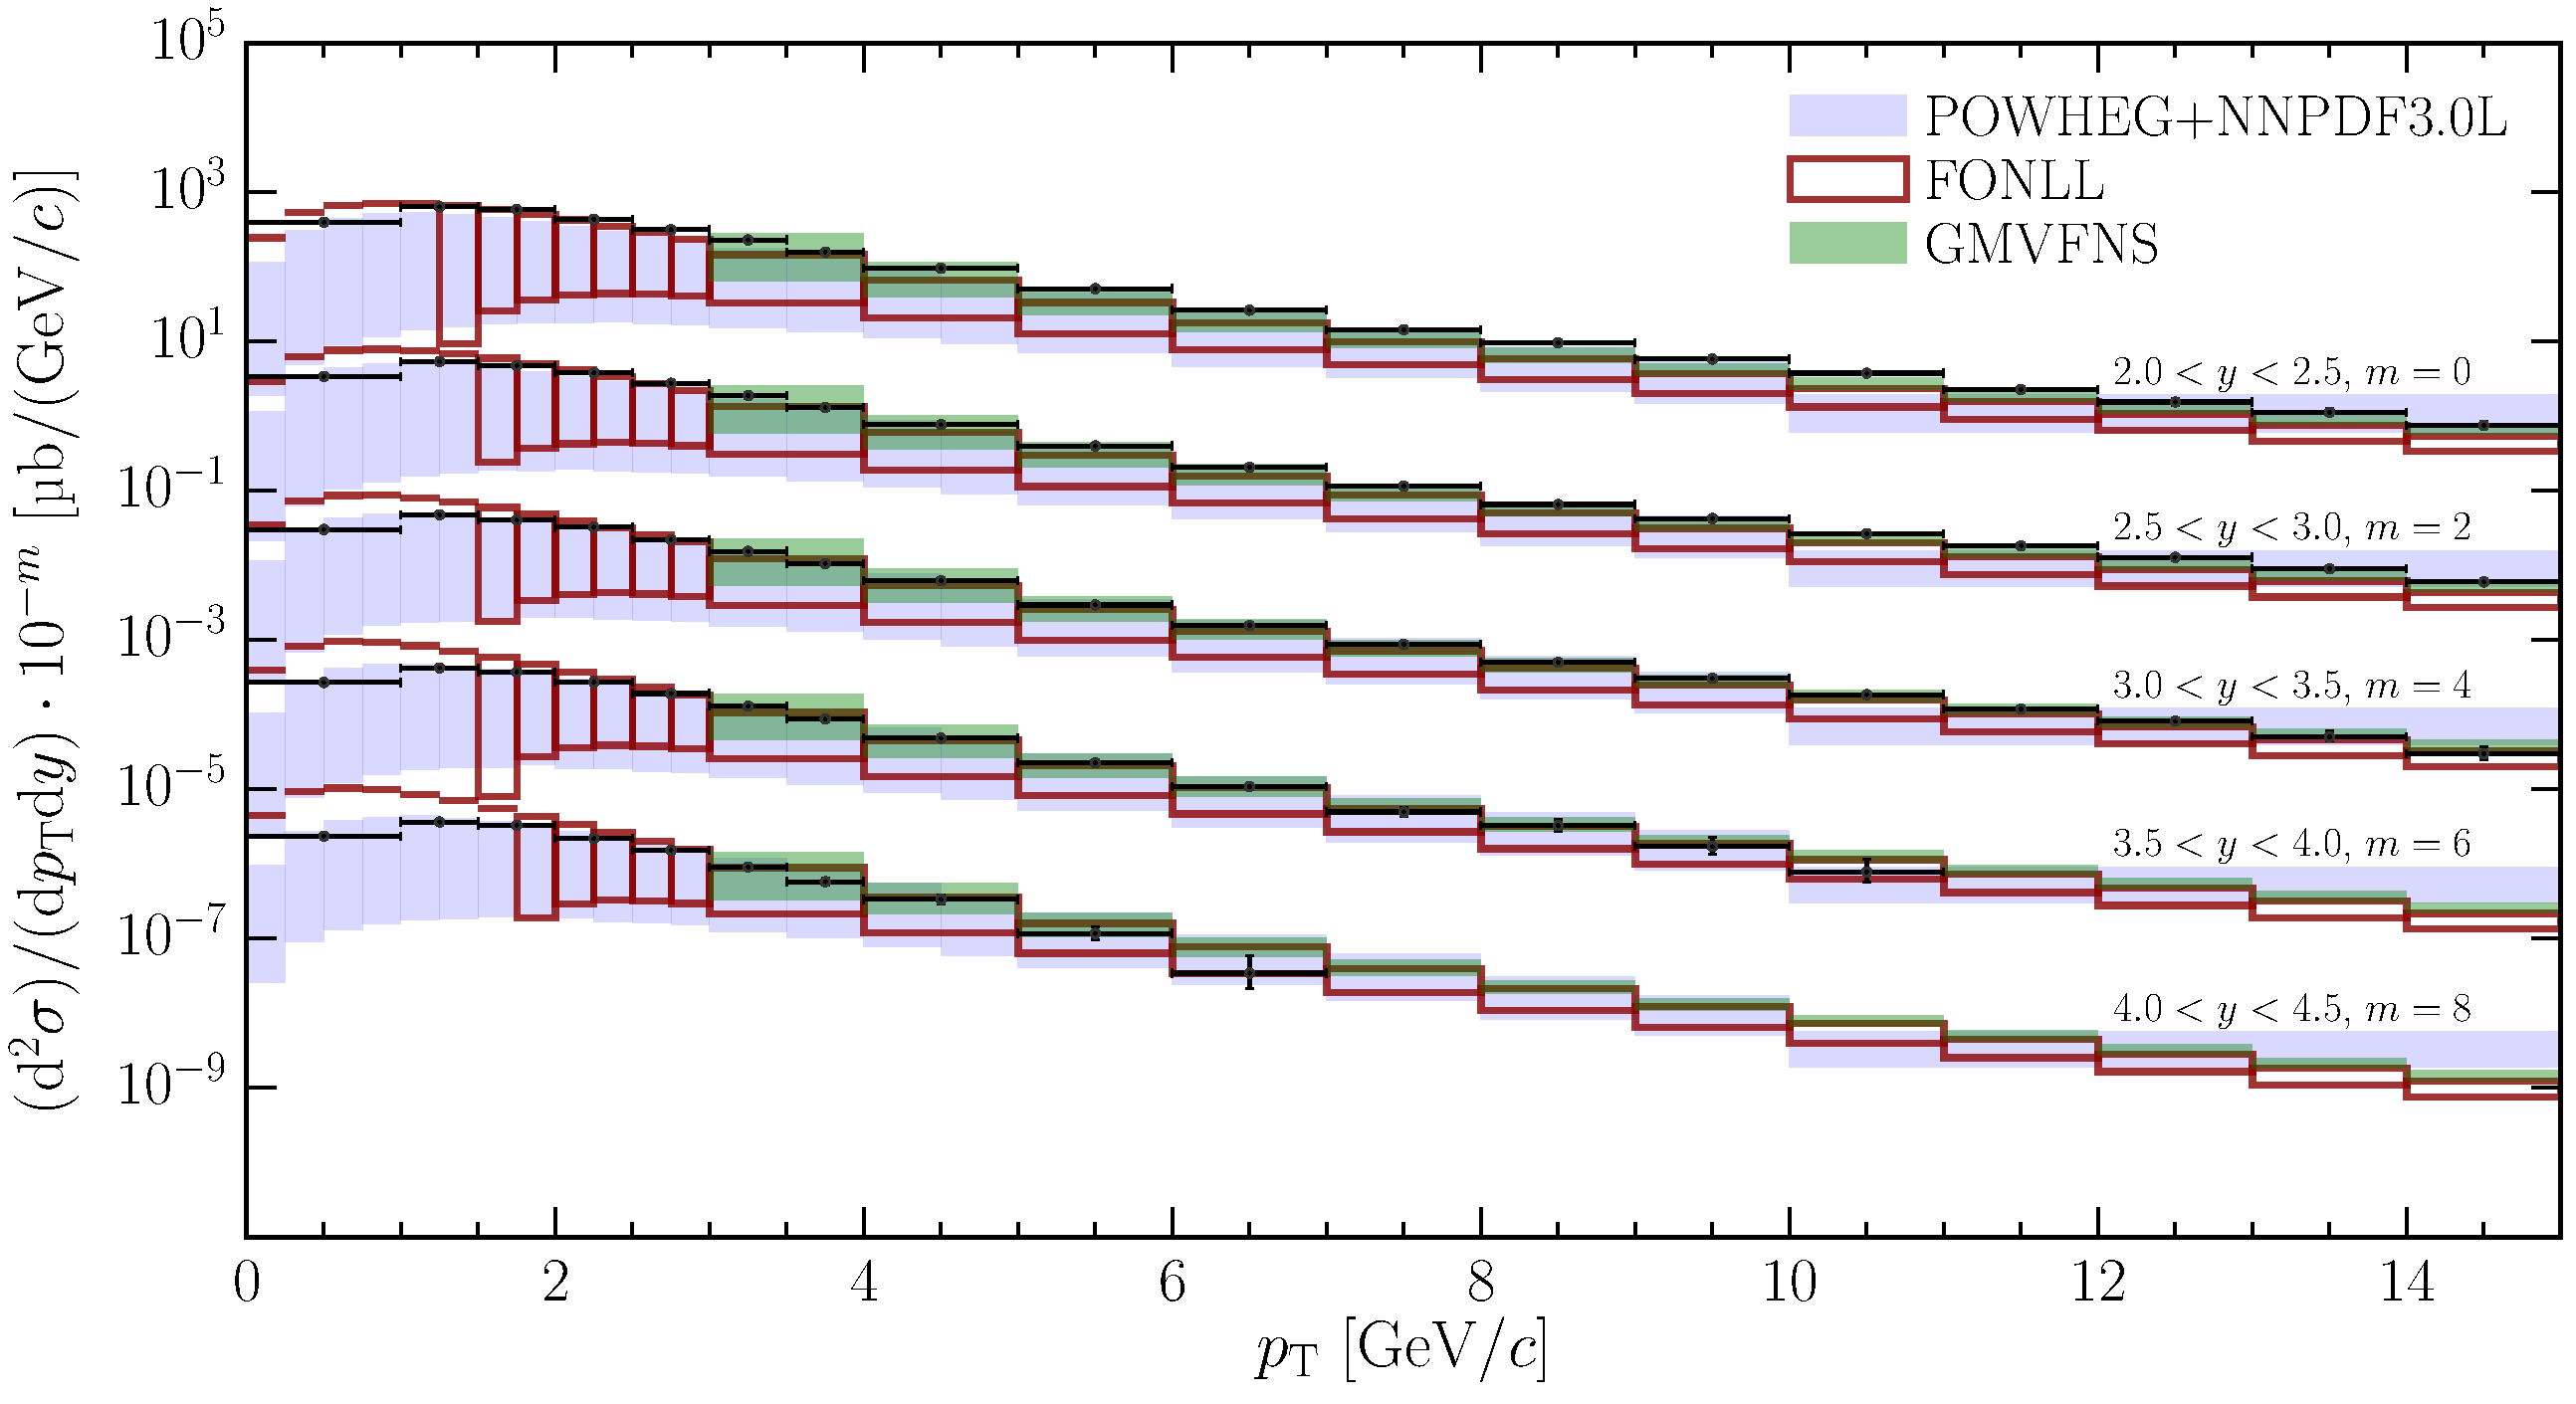
\includegraphics[width=\textwidth]{production/results/D0_double_differential}
    \caption{\PDzero}
    \label{fig:prod:results:double_differential:D0}
  \end{subfigure}
  \begin{subfigure}[b]{\textwidth}
    \centering
    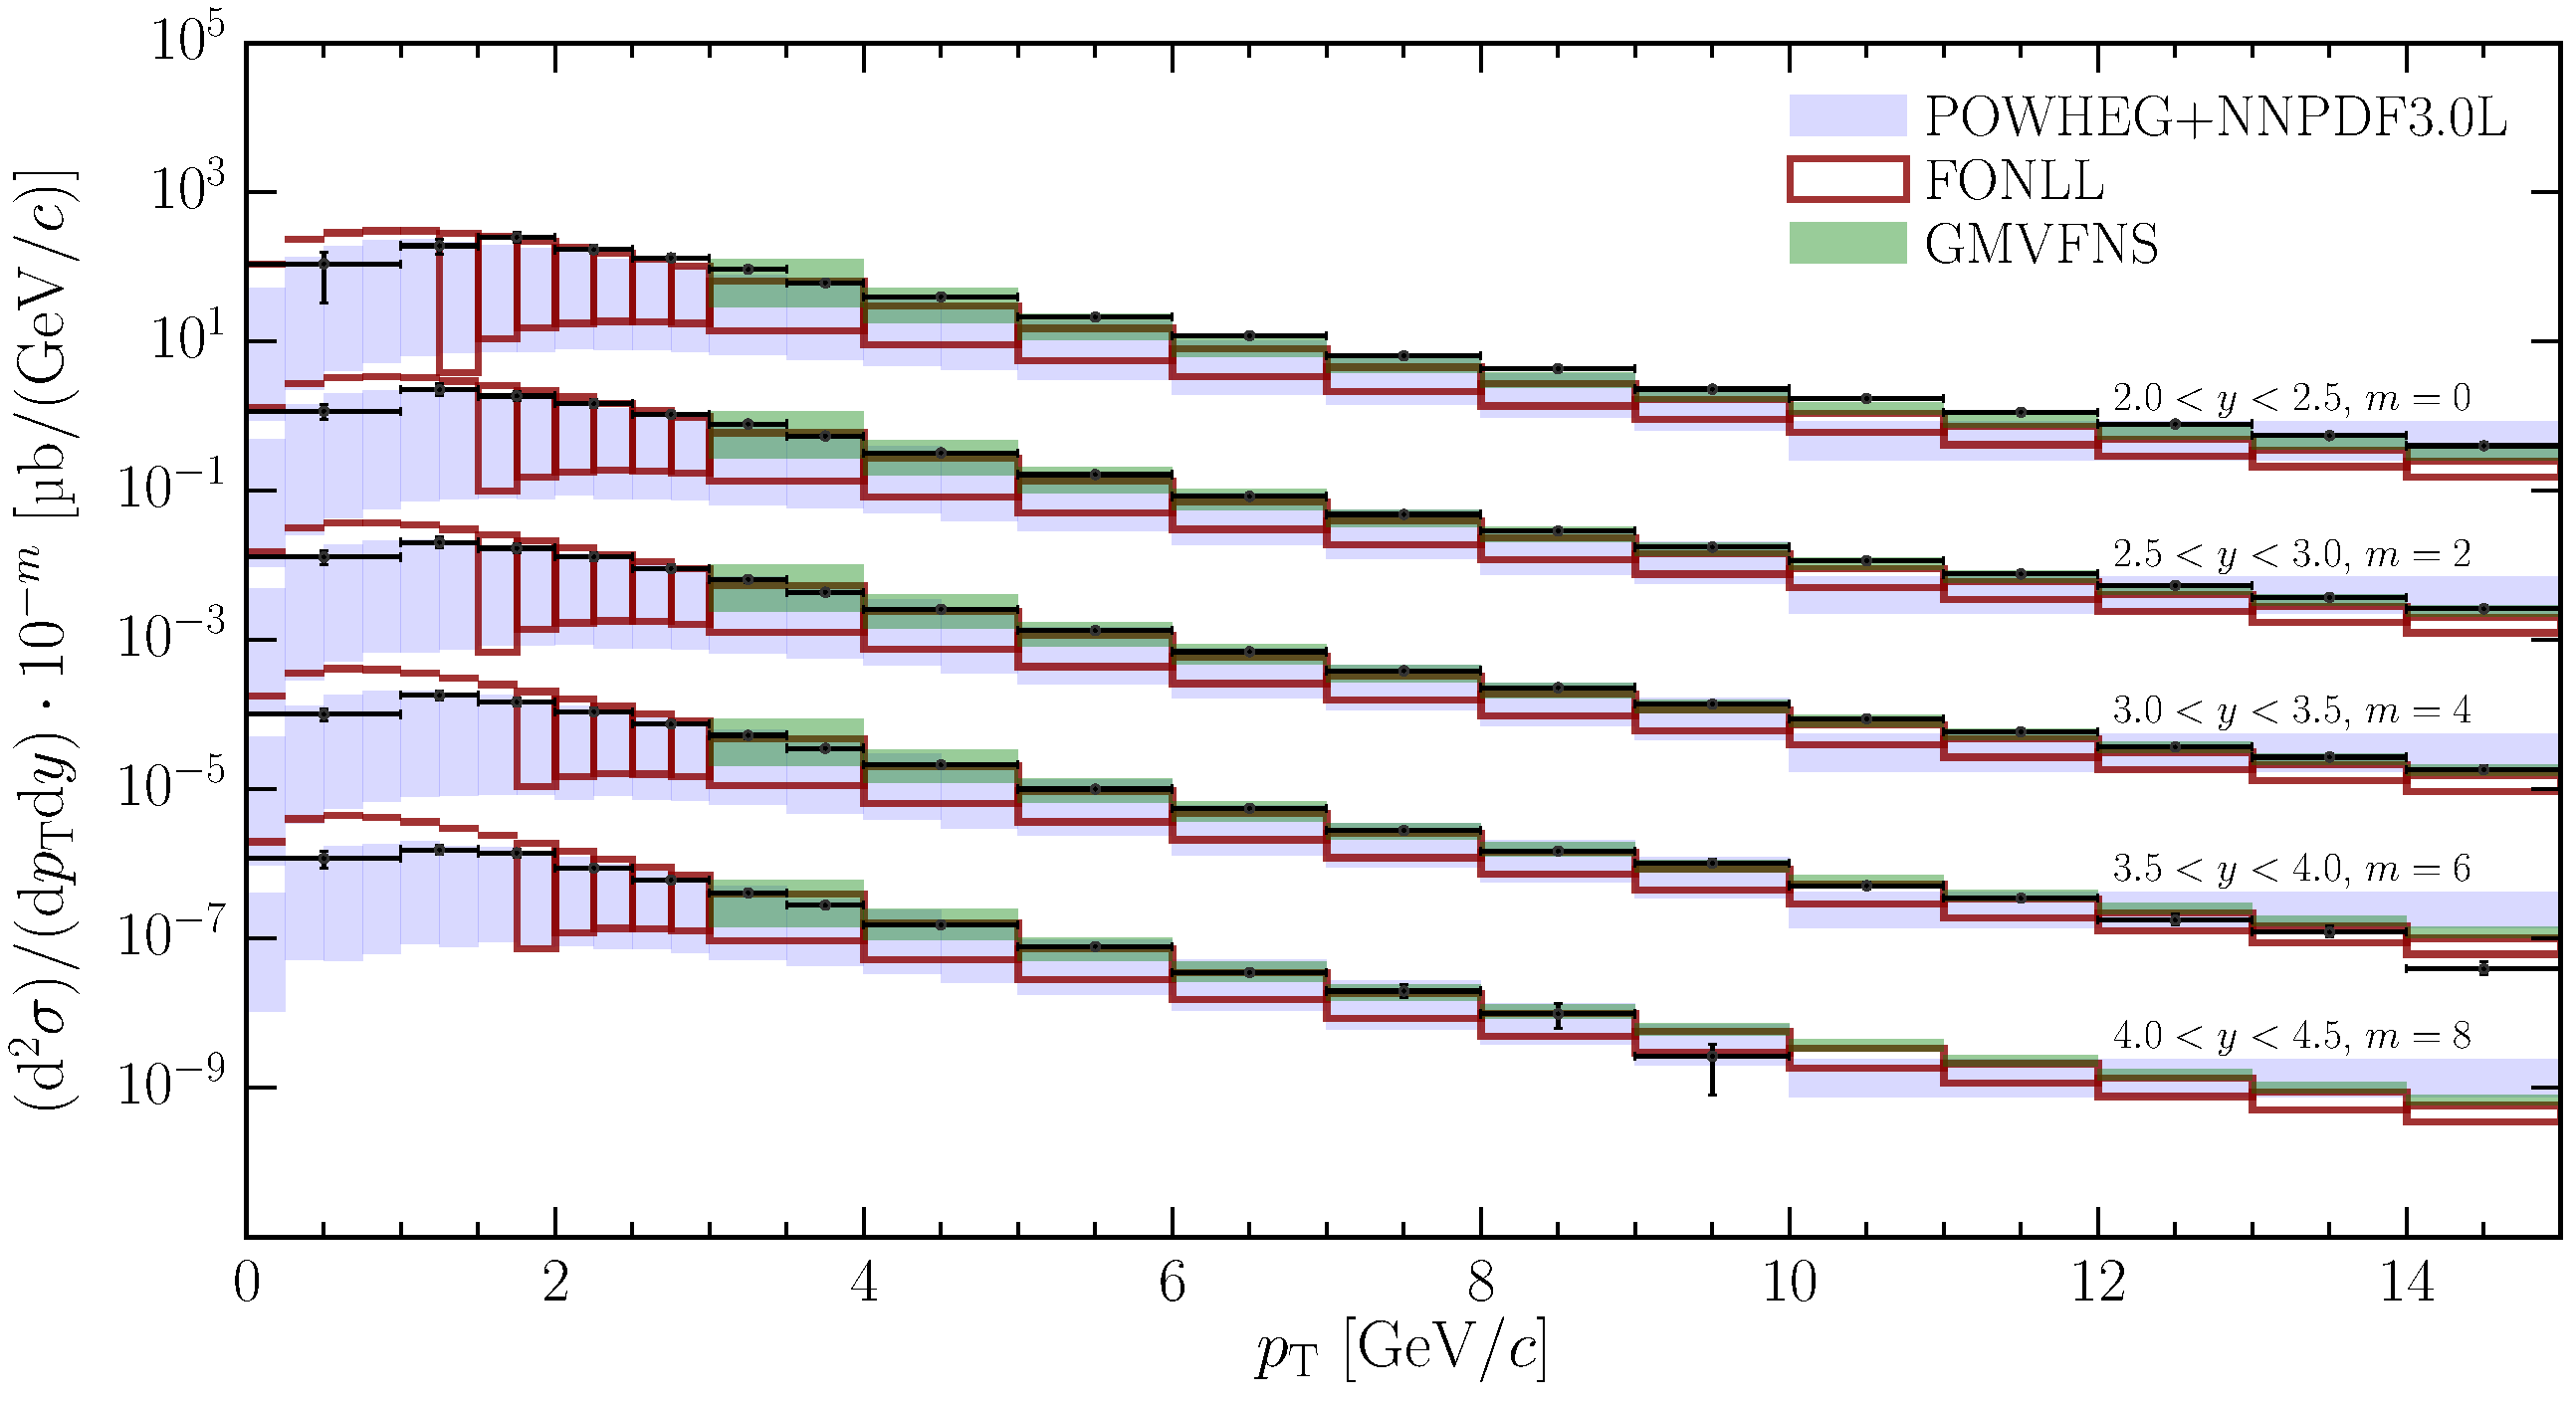
\includegraphics[width=\textwidth]{production/results/Dp_double_differential}
    \caption{\PDplus}
    \label{fig:prod:results:double_differential:Dp}
  \end{subfigure}
  \caption{%
    Measurements and predictions for the absolute prompt \PDzero
    (\subref*{fig:prod:results:double_differential:D0}) and \PDplus
    (\subref*{fig:prod:results:double_differential:Dp}) cross-sections at
    \sqrtseq{13}.
    Each set of measurements and predictions in a given rapidity bin is offset
    by a multiplicative factor $10^{-m}$, where the factor $m$ is shown on the
    plots.
    The boxes indicate the $\pm1\sigma$ uncertainty band on the theory
    predictions.
    In cases where this band spans more than two orders of magnitude only its
    upper edge is indicated.
  }
  \label{fig:prod:results:double_differential:D0_Dp}
\end{figure}

\begin{figure}
  \begin{subfigure}[b]{\textwidth}
    \centering
    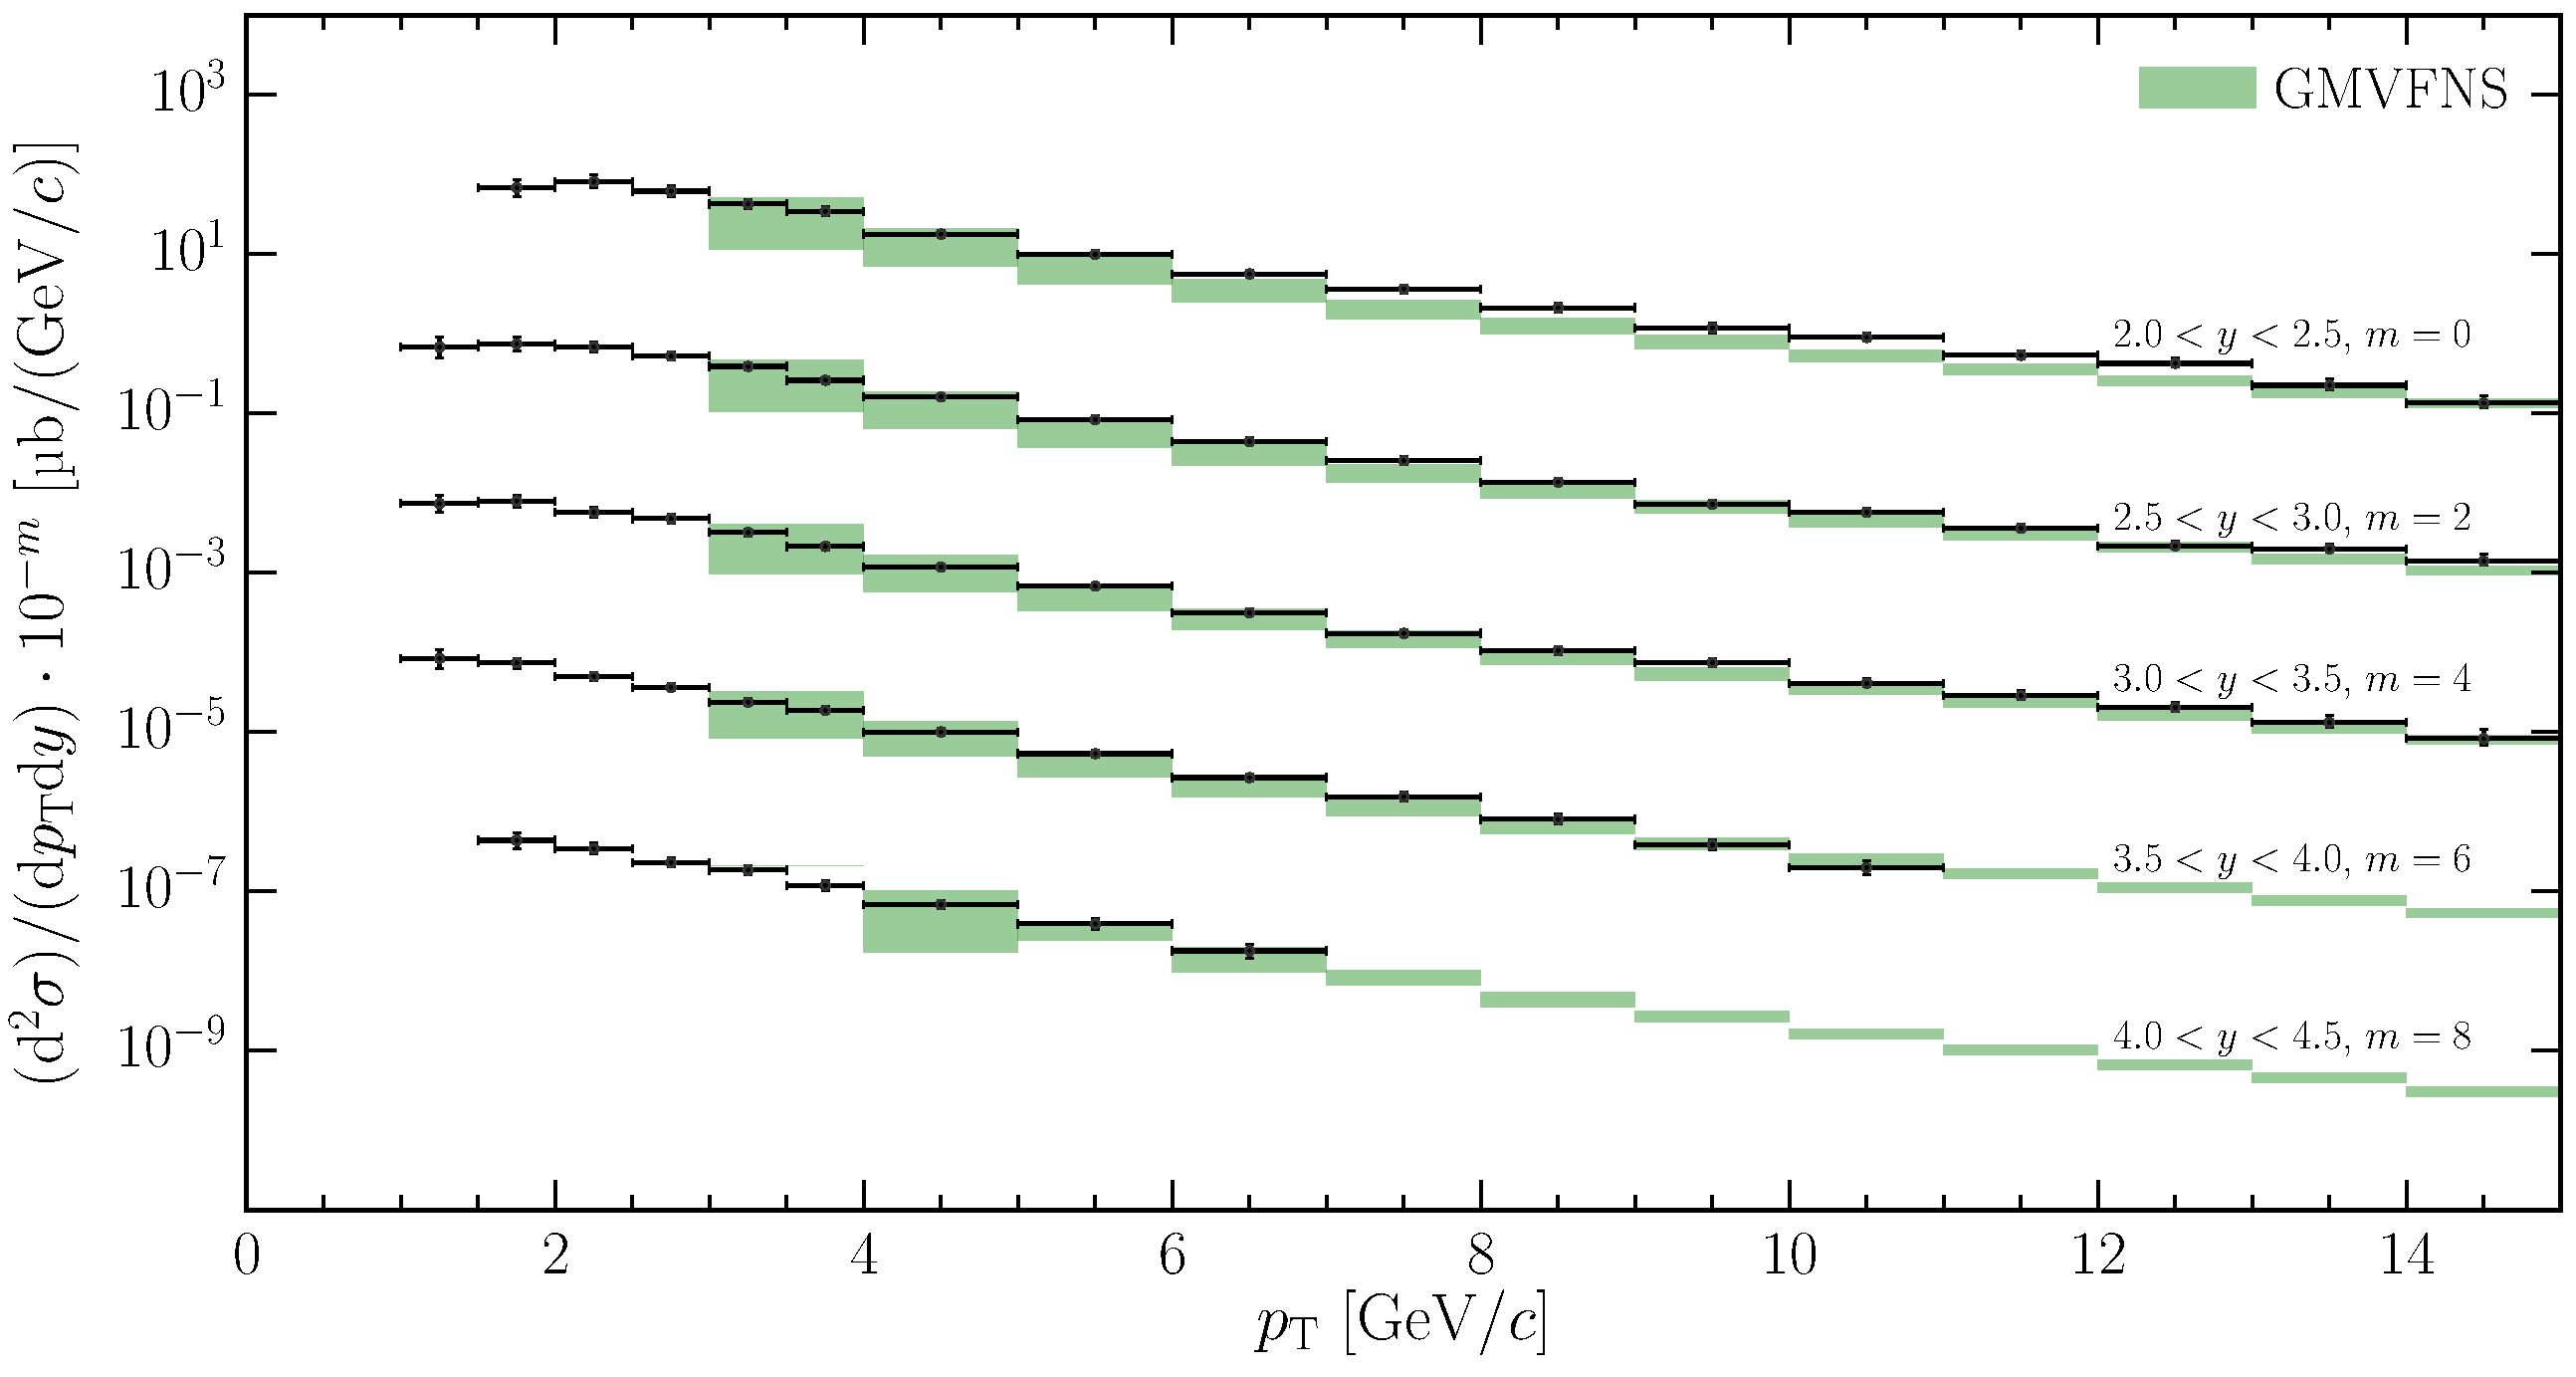
\includegraphics[width=\textwidth]{production/results/Ds_double_differential}
    \caption{\PDsplus}
    \label{fig:prod:results:double_differential:Ds}
  \end{subfigure}
  \begin{subfigure}[b]{\textwidth}
    \centering
    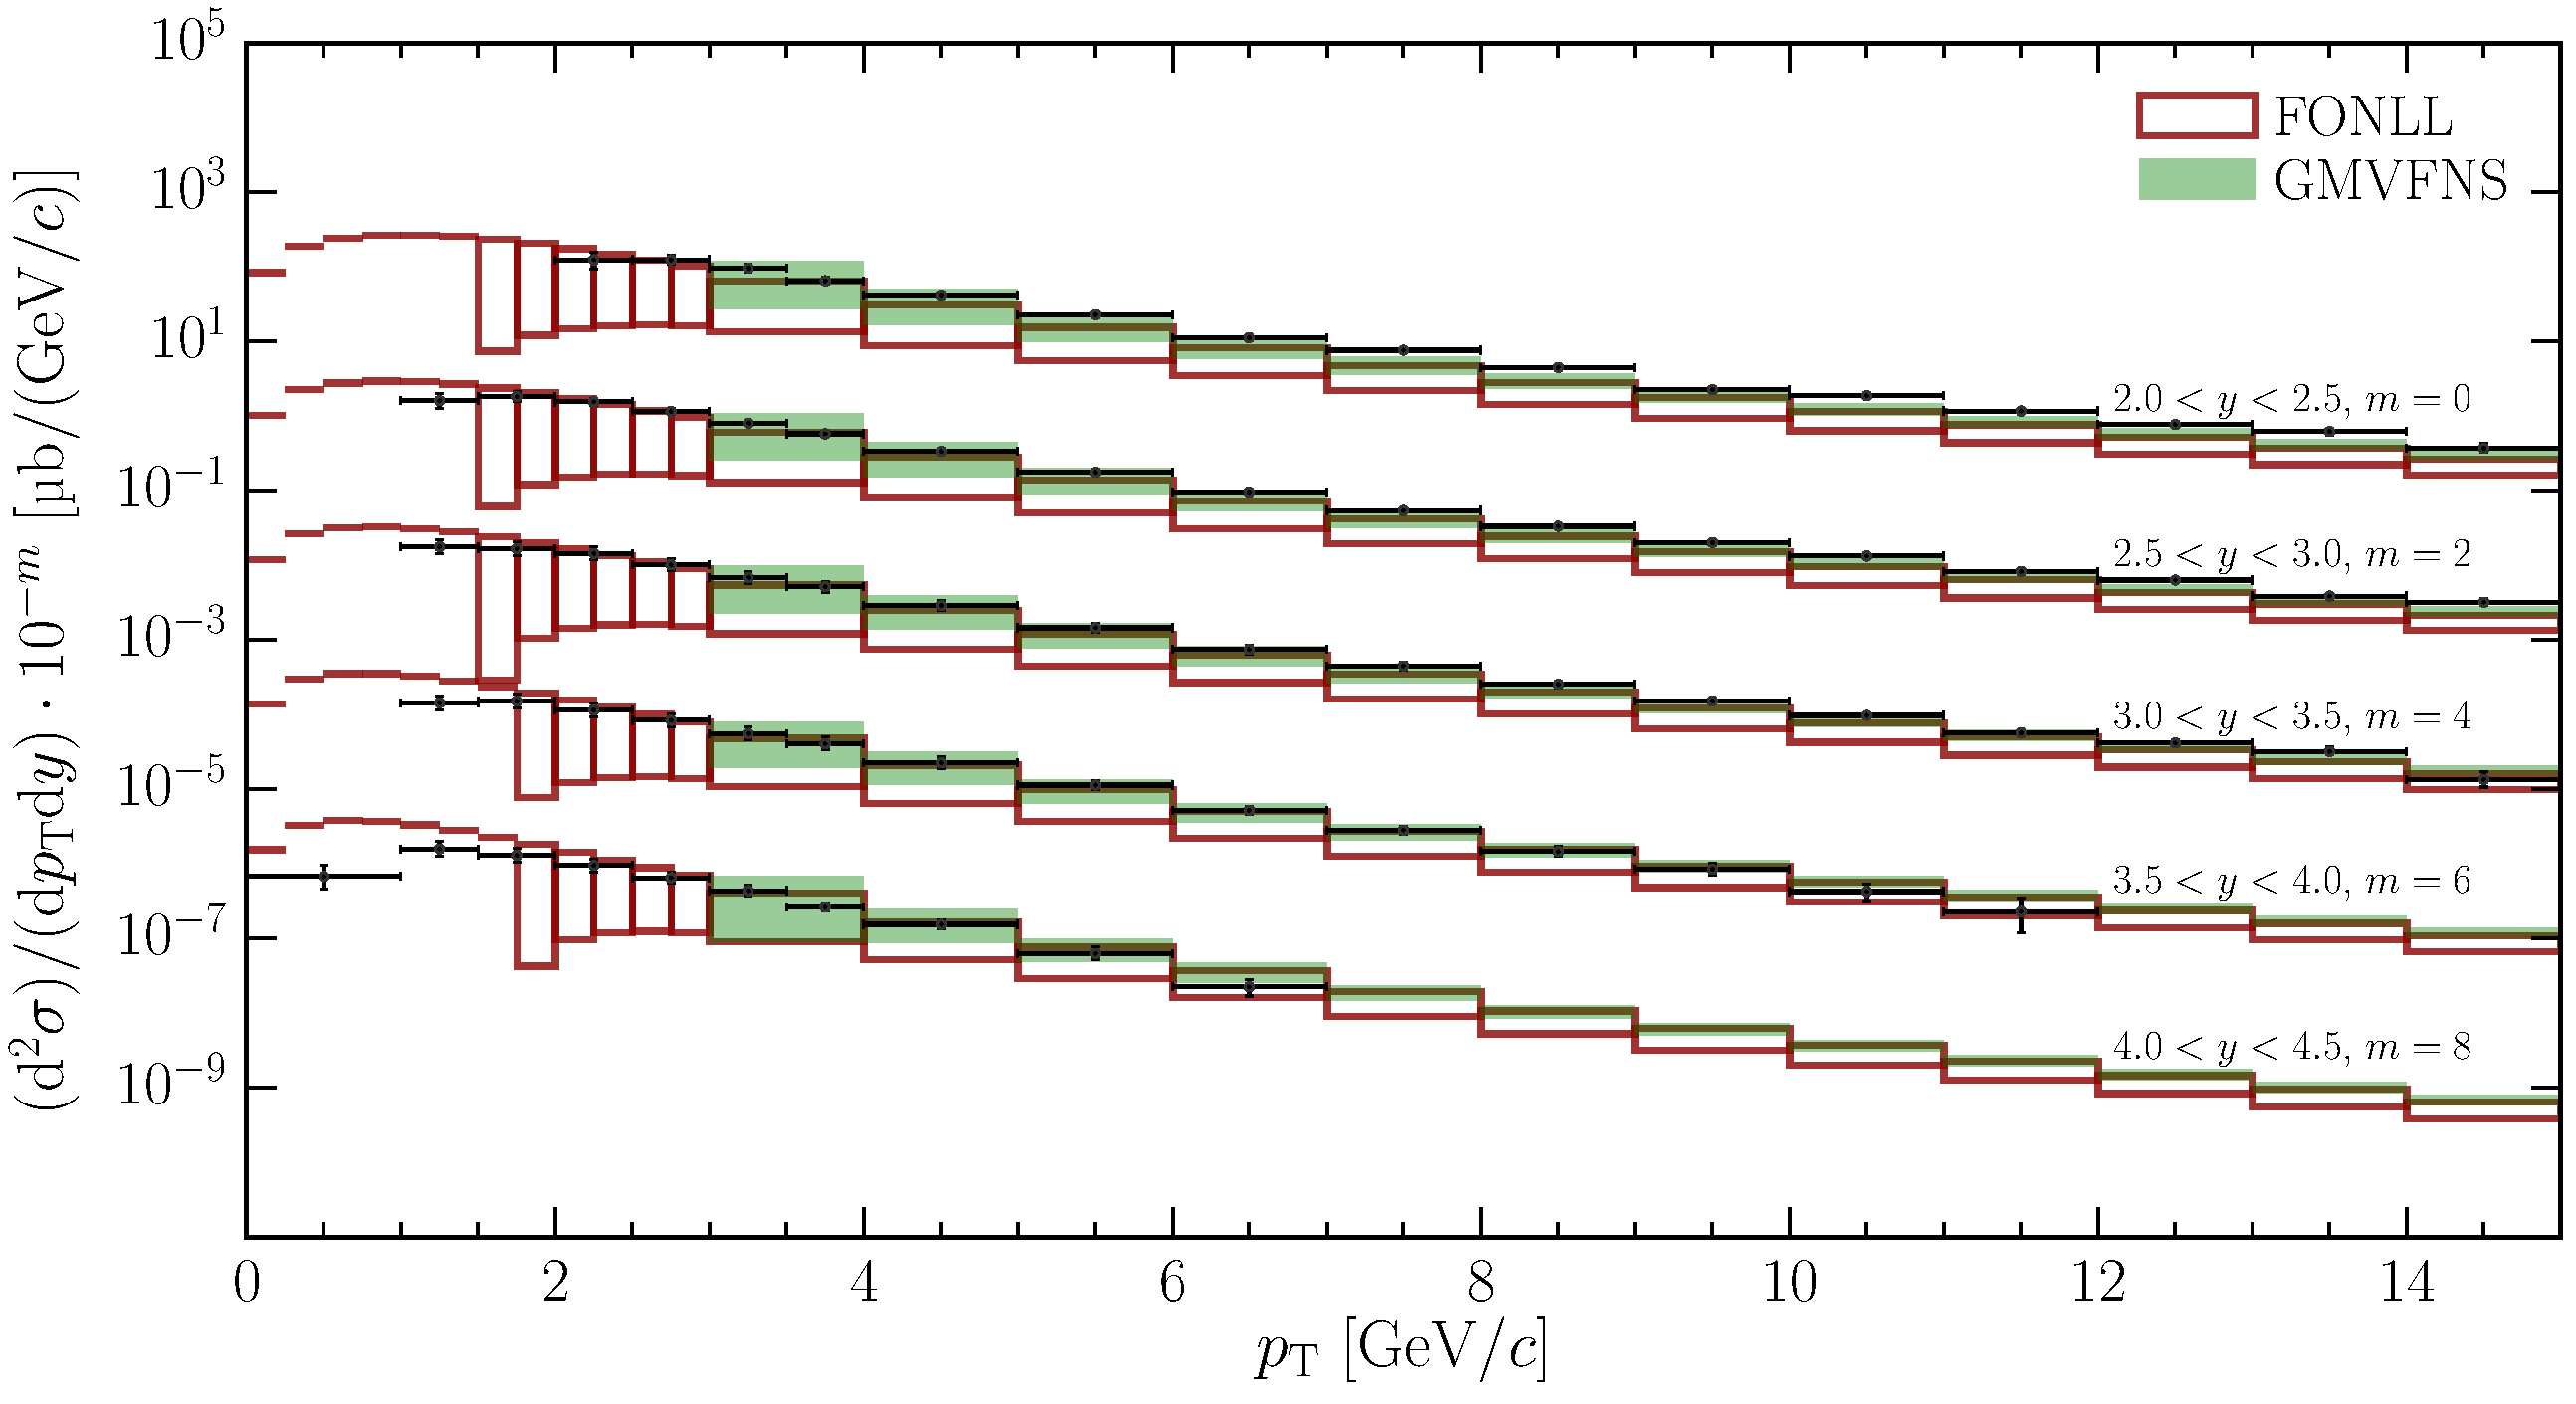
\includegraphics[width=\textwidth]{production/results/Dst_double_differential}
    \caption{\PDstarp}
    \label{fig:prod:results:double_differential:Dst}
  \end{subfigure}
  \caption{%
    Measurements and predictions for the absolute prompt \PDsplus
    (\subref*{fig:prod:results:double_differential:Ds}) and \PDstarp
    (\subref*{fig:prod:results:double_differential:Dst}) cross-sections at
    \sqrtseq{13}.
    Each set of measurements and predictions in a given rapidity bin is offset
    by a multiplicative factor $10^{-m}$, where the factor $m$ is shown on the
    plots.
    The boxes indicate the $\pm1\sigma$ uncertainty band on the theory
    predictions.
    In cases where this band spans more than two orders of magnitude only its
    upper edge is indicated.
  }
  \label{fig:prod:results:double_differential:Ds_Dst}
\end{figure}

\begin{figure}
  \begin{subfigure}[b]{0.5\textwidth}
    \centering
    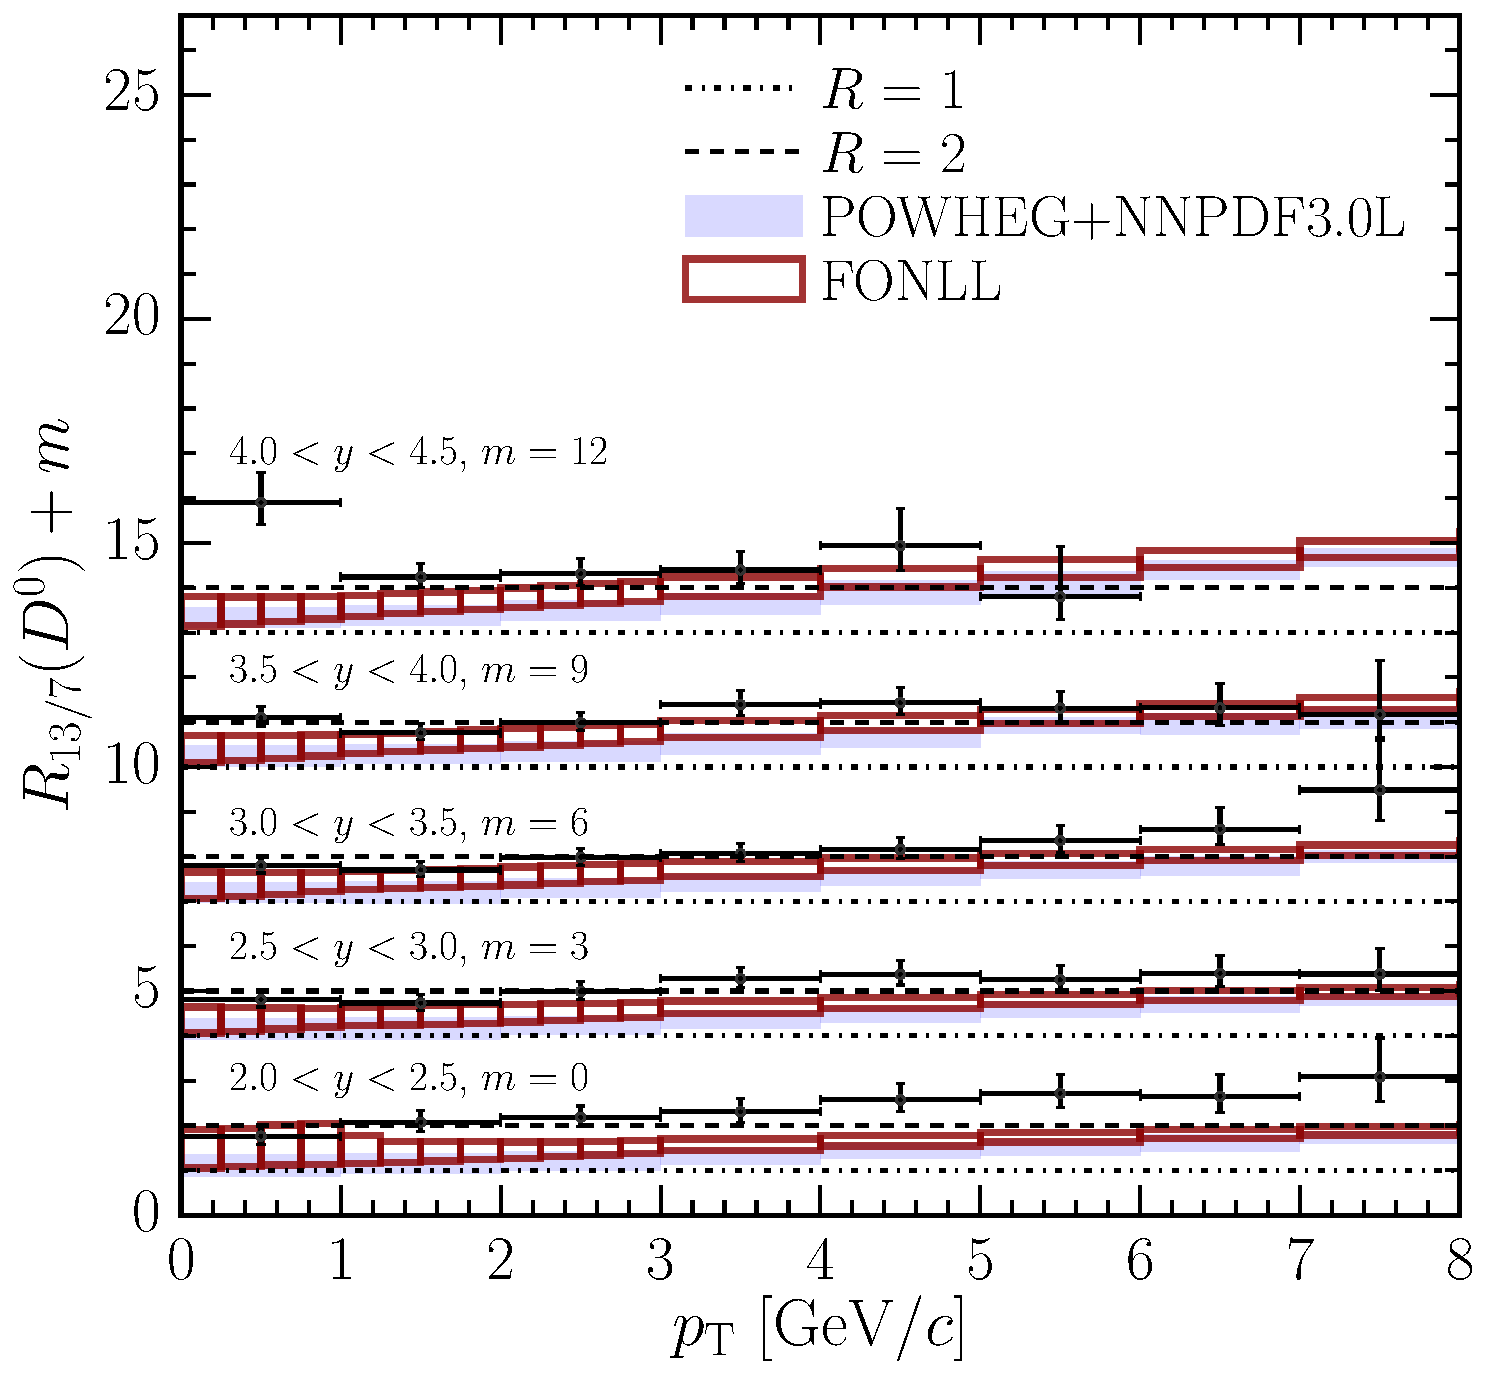
\includegraphics[width=\textwidth]{production/results/D0_ratio_with_2010}
    \caption{\PDzero}
    \label{fig:prod:results:ratio_7tev:D0}
  \end{subfigure}
  \begin{subfigure}[b]{0.5\textwidth}
    \centering
    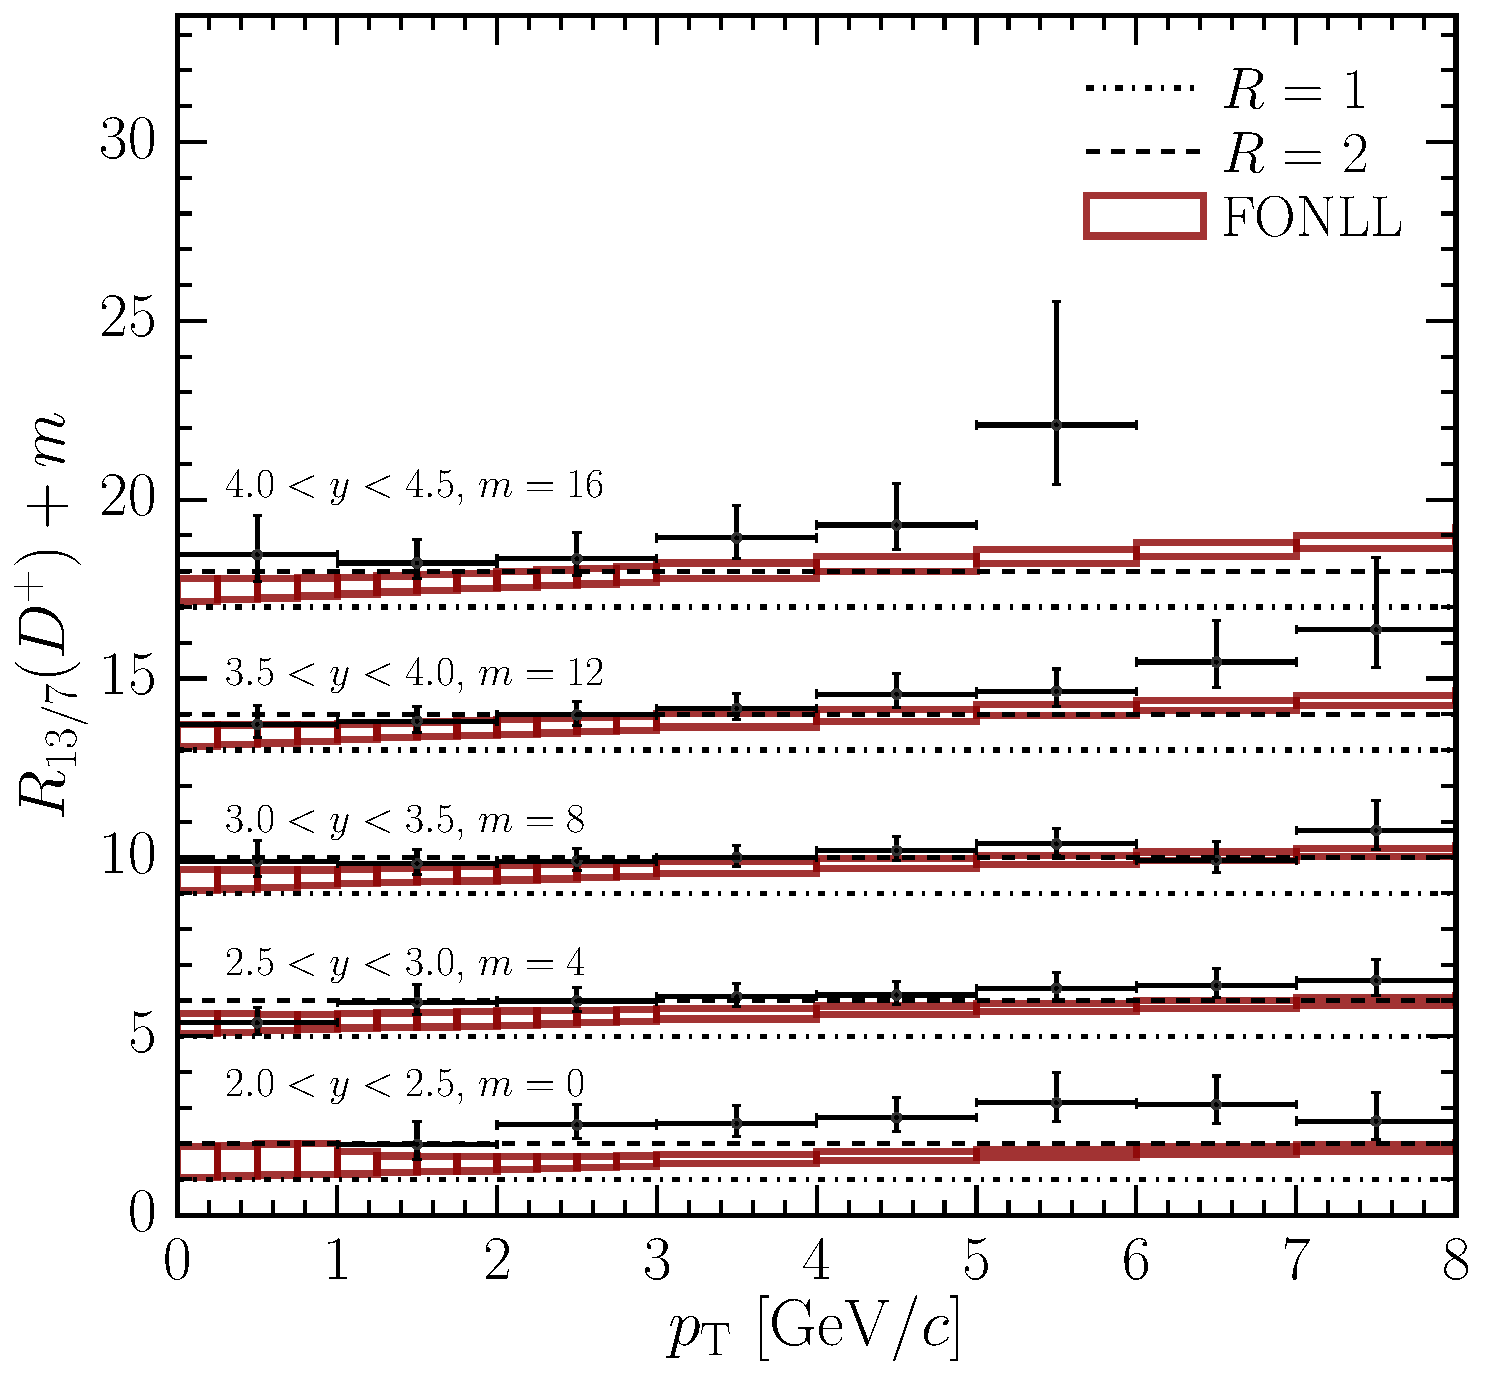
\includegraphics[width=\textwidth]{production/results/Dp_ratio_with_2010}
    \caption{\PDplus}
    \label{fig:prod:results:ratio_7tev:Dp}
  \end{subfigure}
  \begin{subfigure}[b]{0.5\textwidth}
    \centering
    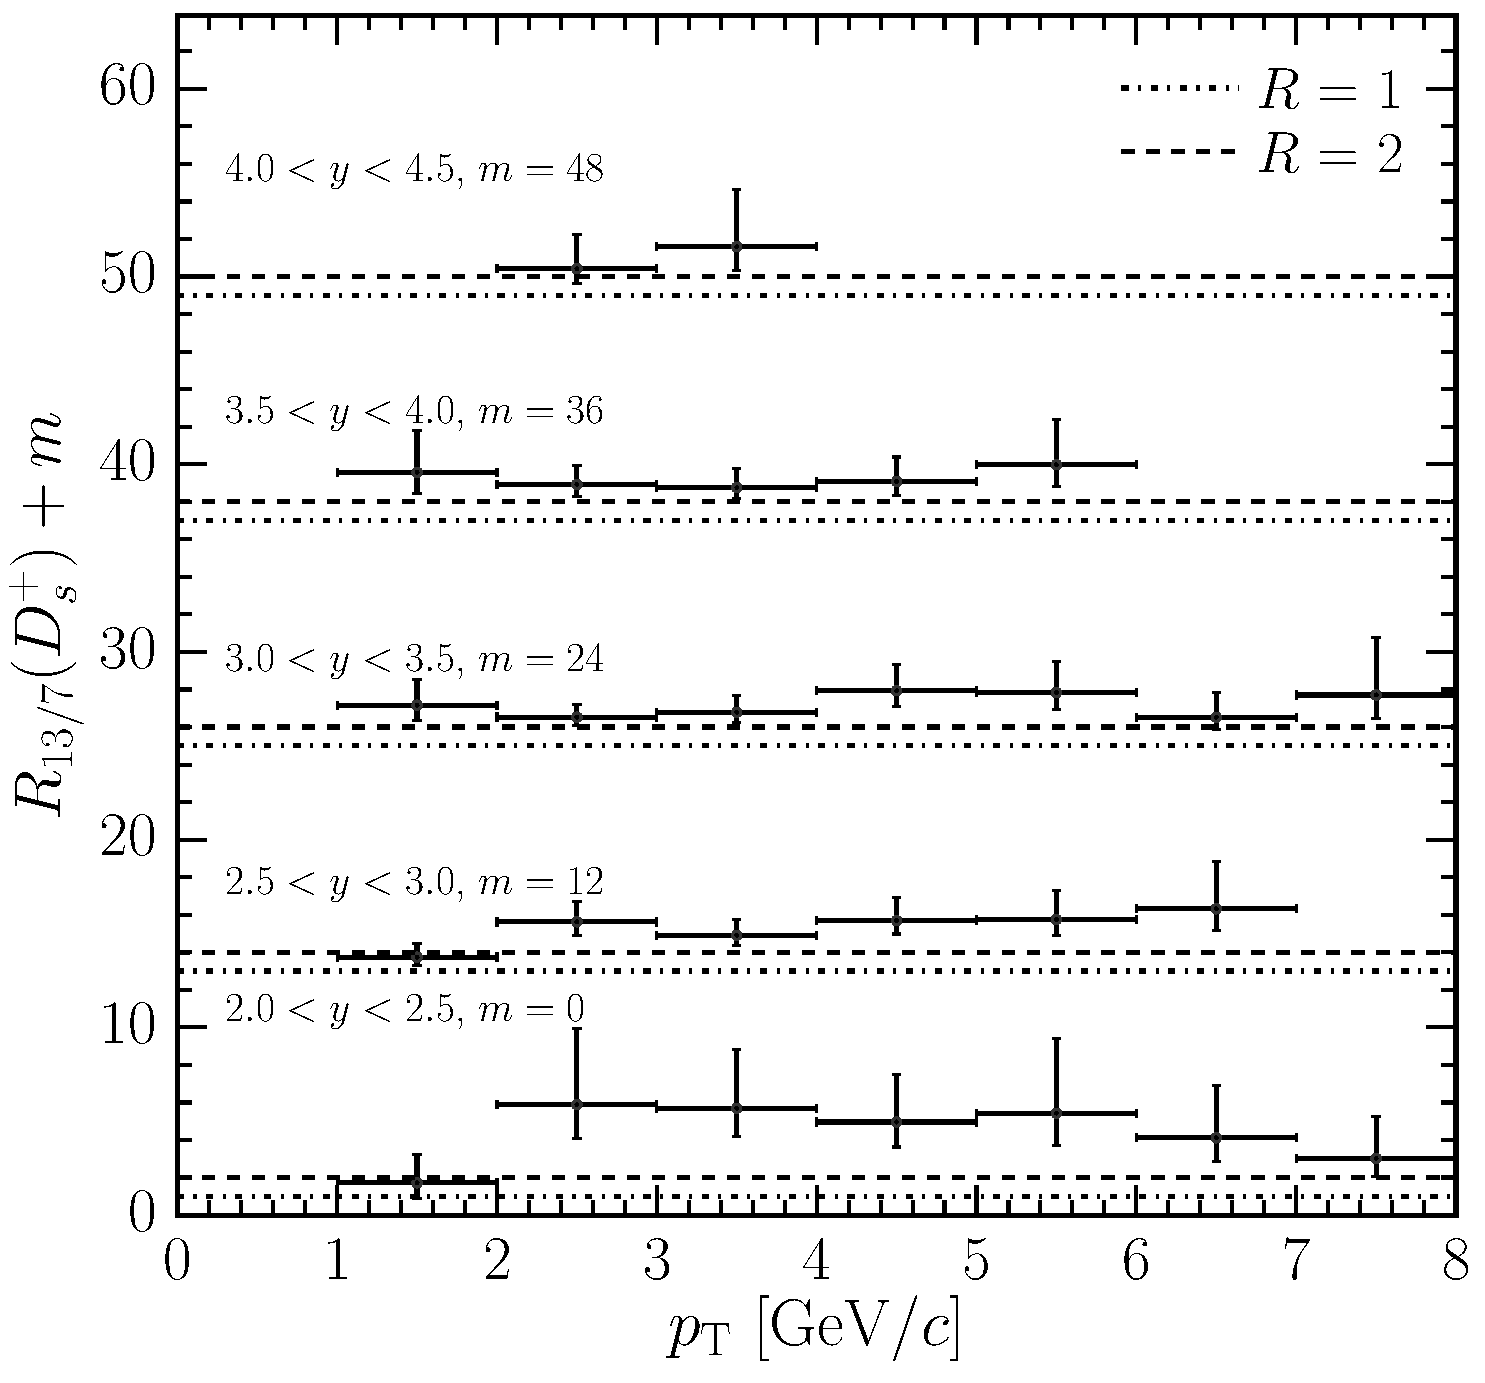
\includegraphics[width=\textwidth]{production/results/Ds_ratio_with_2010}
    \caption{\PDsplus}
    \label{fig:prod:results:ratio_7tev:Ds}
  \end{subfigure}
  \begin{subfigure}[b]{0.5\textwidth}
    \centering
    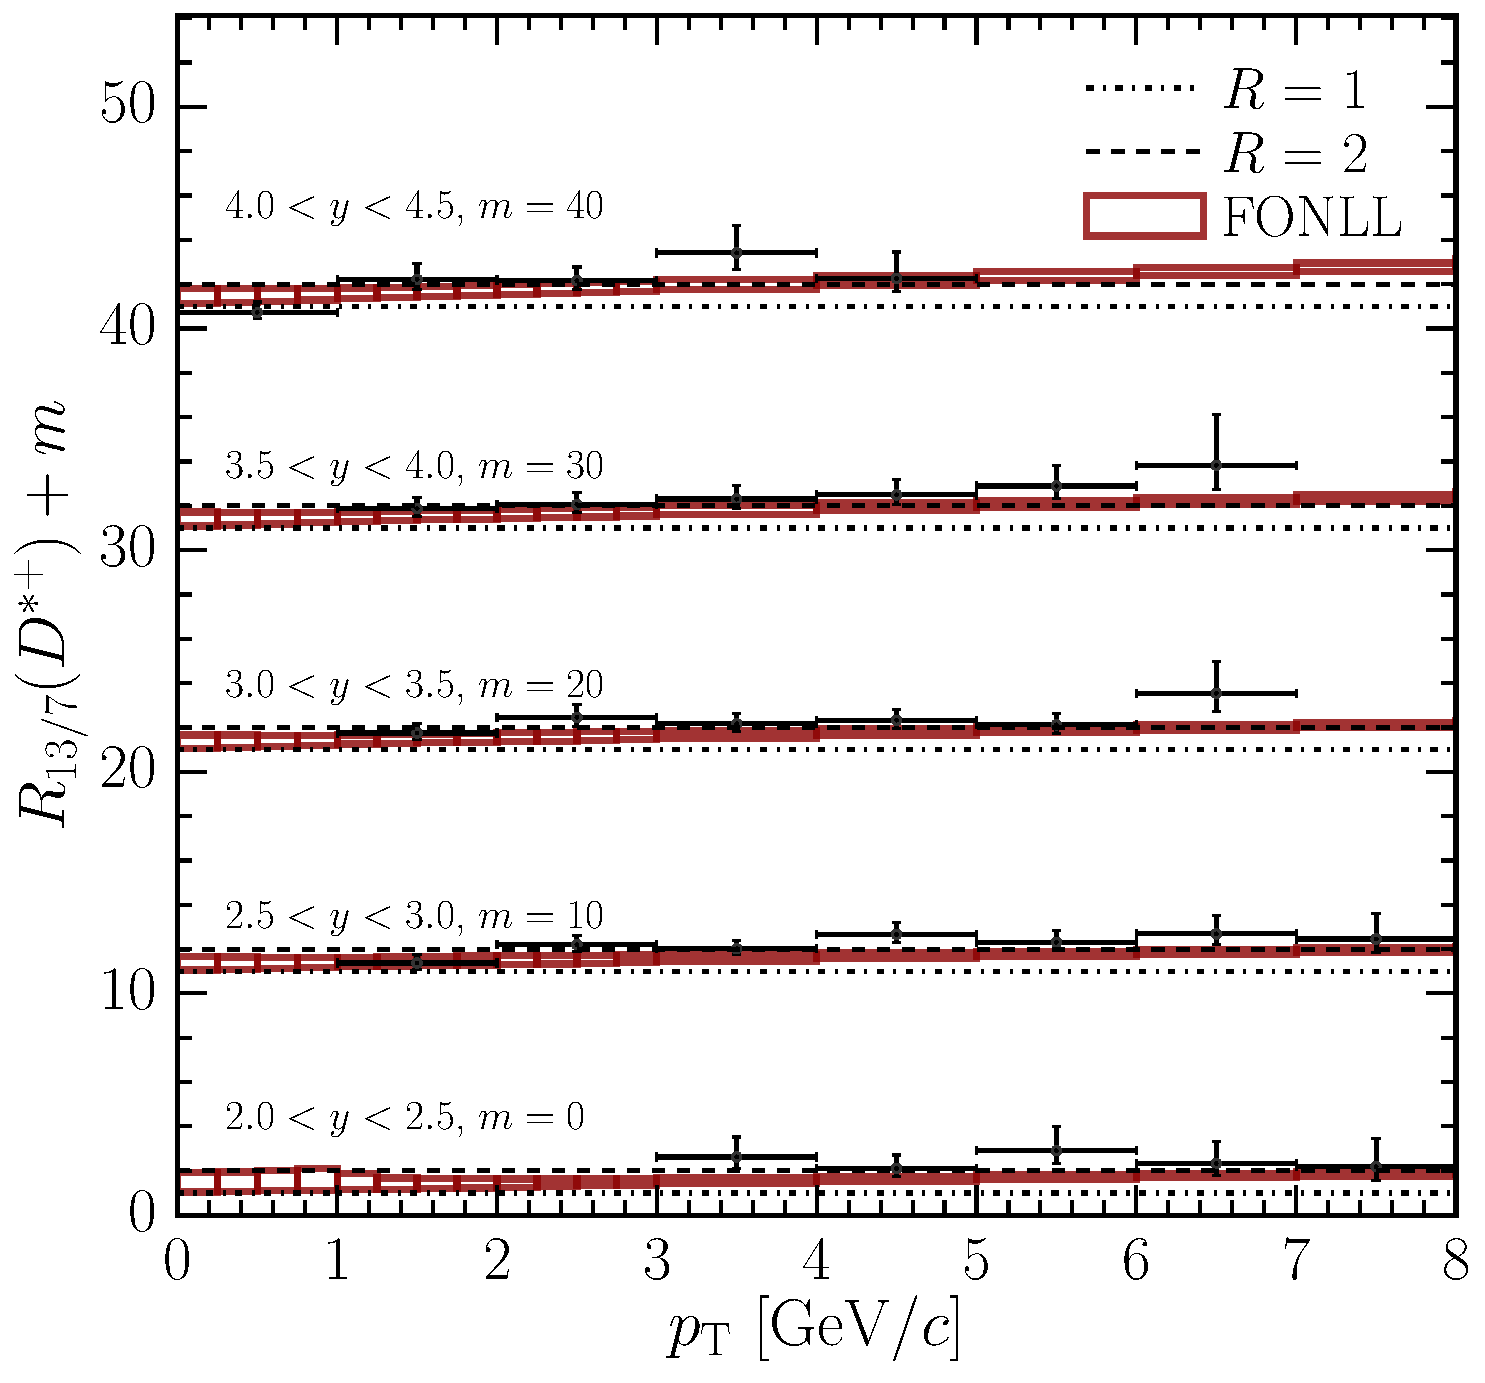
\includegraphics[width=\textwidth]{production/results/Dst_ratio_with_2010}
    \caption{\PDstarp}
    \label{fig:prod:results:ratio_7tev:Dst}
  \end{subfigure}
  \caption{%
    Measurements and predictions of the prompt \PDzero
    (\subref*{fig:prod:results:ratio_7tev:D0}), \PDplus
    (\subref*{fig:prod:results:ratio_7tev:Dp}), \PDsplus
    (\subref*{fig:prod:results:ratio_7tev:Ds}), and \PDstarp
    (\subref*{fig:prod:results:ratio_7tev:Dst}) cross-section ratios
    \resultratio{13}{7}.
    Each set of measurements and predictions in a given rapidity bin is offset
    by an additive factor $m$ shown on the plots.
    The dash-dotted lines indicate the unit ratio for each of the rapidity
    intervals and the dashed lines indicate a ratio of two.
    No prediction is available for the \PDsplus ratio.
  }
  \label{fig:prod:results:ratio_7tev}
\end{figure}

\begin{figure}
  \begin{subfigure}[b]{0.5\textwidth}
    \centering
    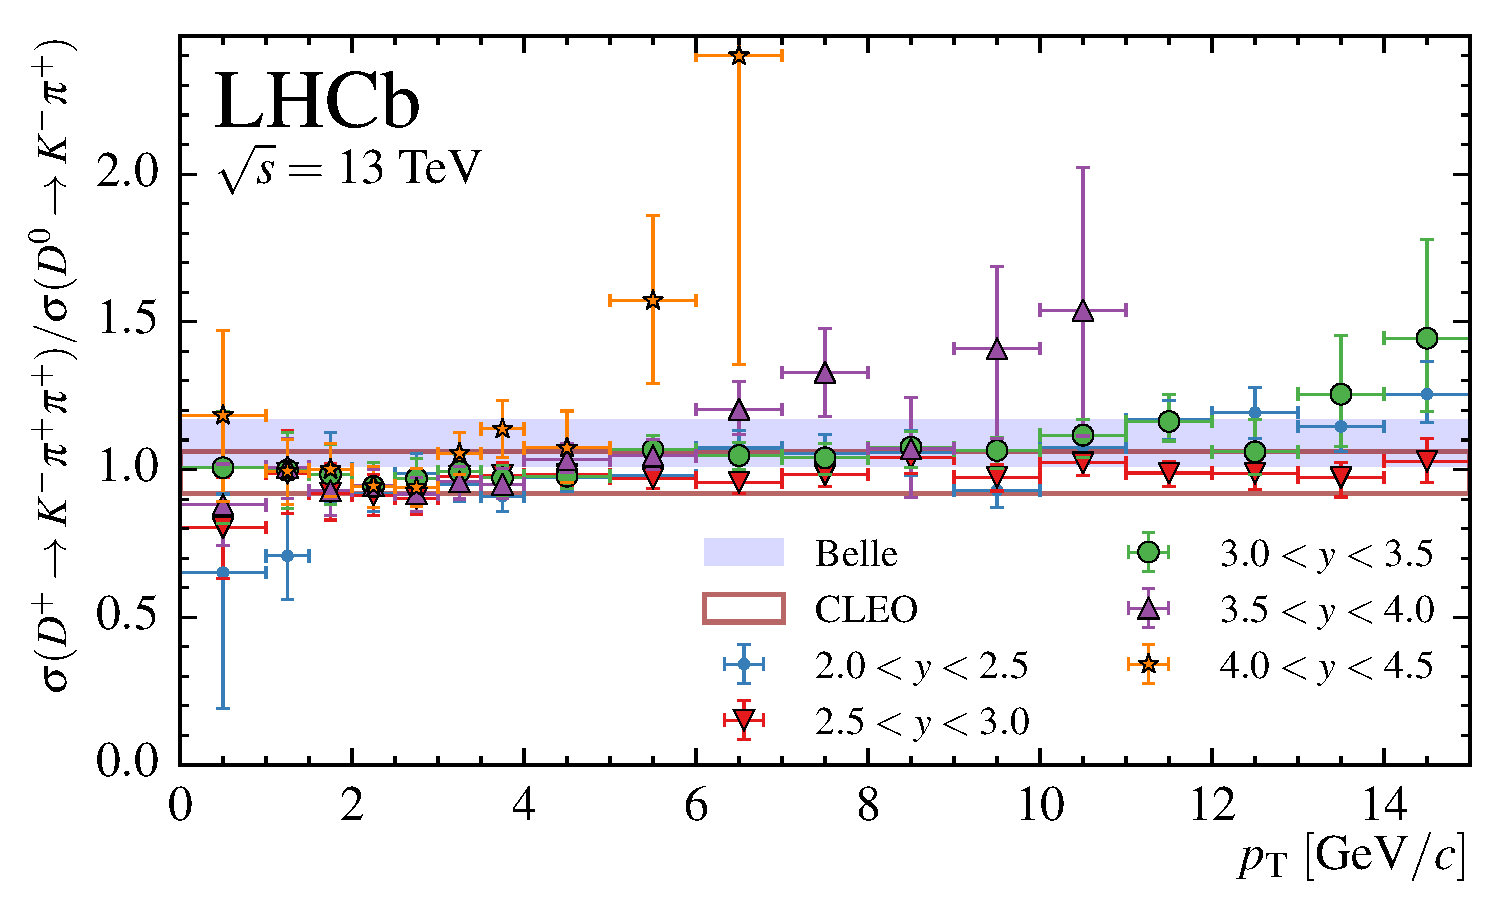
\includegraphics[width=\textwidth]{production/results/Dp_ratio_with_D0}
    \caption{\resultratio{\PDplus}{\PDzero}}
    \label{fig:prod:results:ratio_mesons:Dp_D0}
  \end{subfigure}
  \begin{subfigure}[b]{0.5\textwidth}
    \centering
    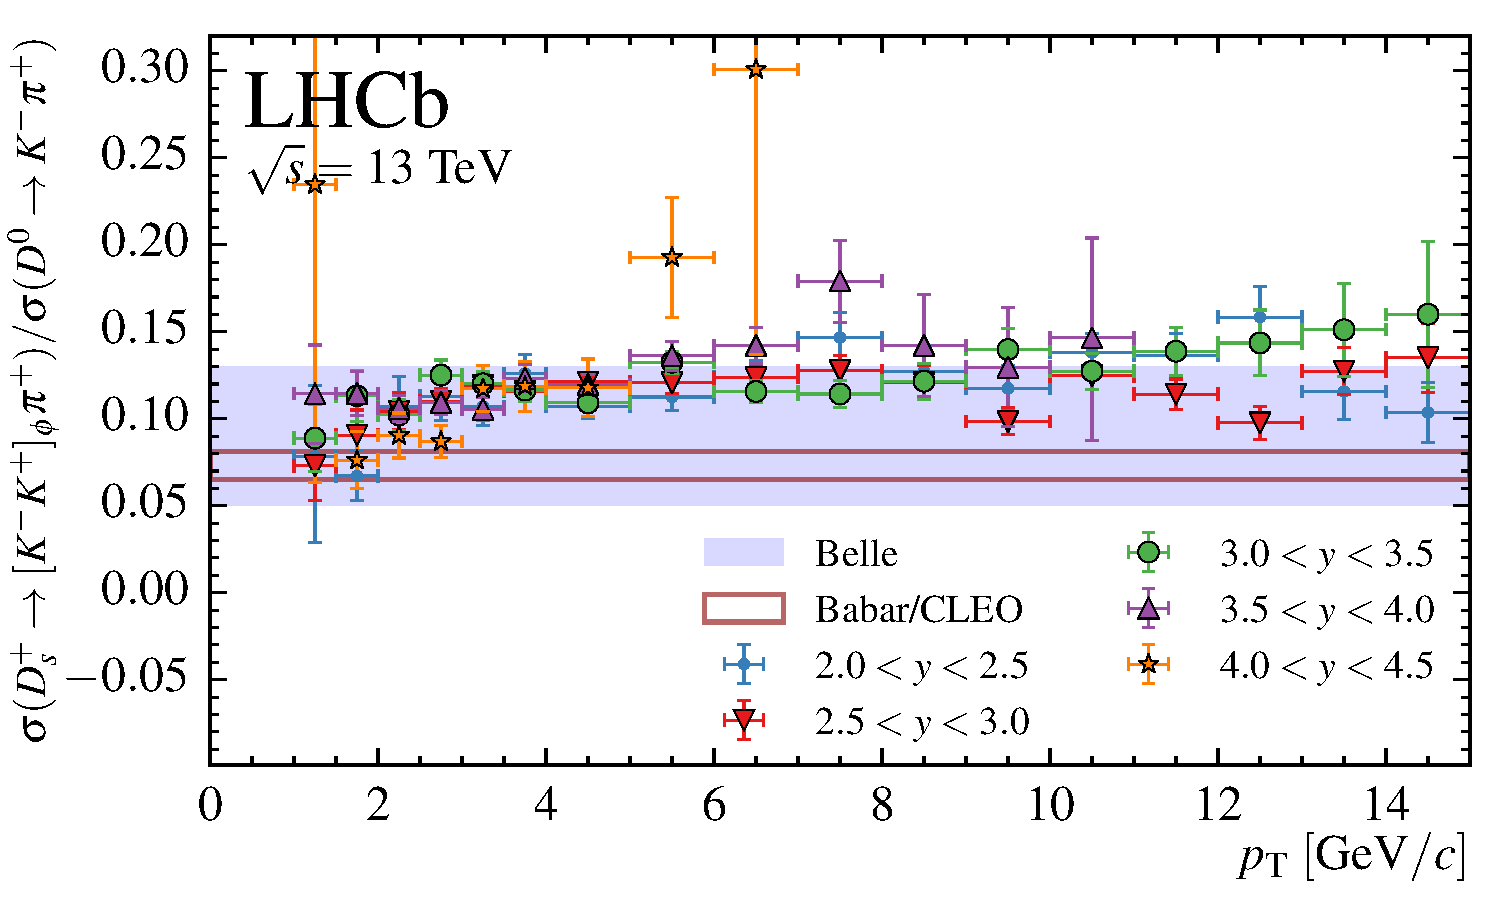
\includegraphics[width=\textwidth]{production/results/Ds_ratio_with_D0}
    \caption{\resultratio{\PDsplus}{\PDzero}}
    \label{fig:prod:results:ratio_mesons:Ds_D0}
  \end{subfigure}
  \begin{subfigure}[b]{0.5\textwidth}
    \centering
    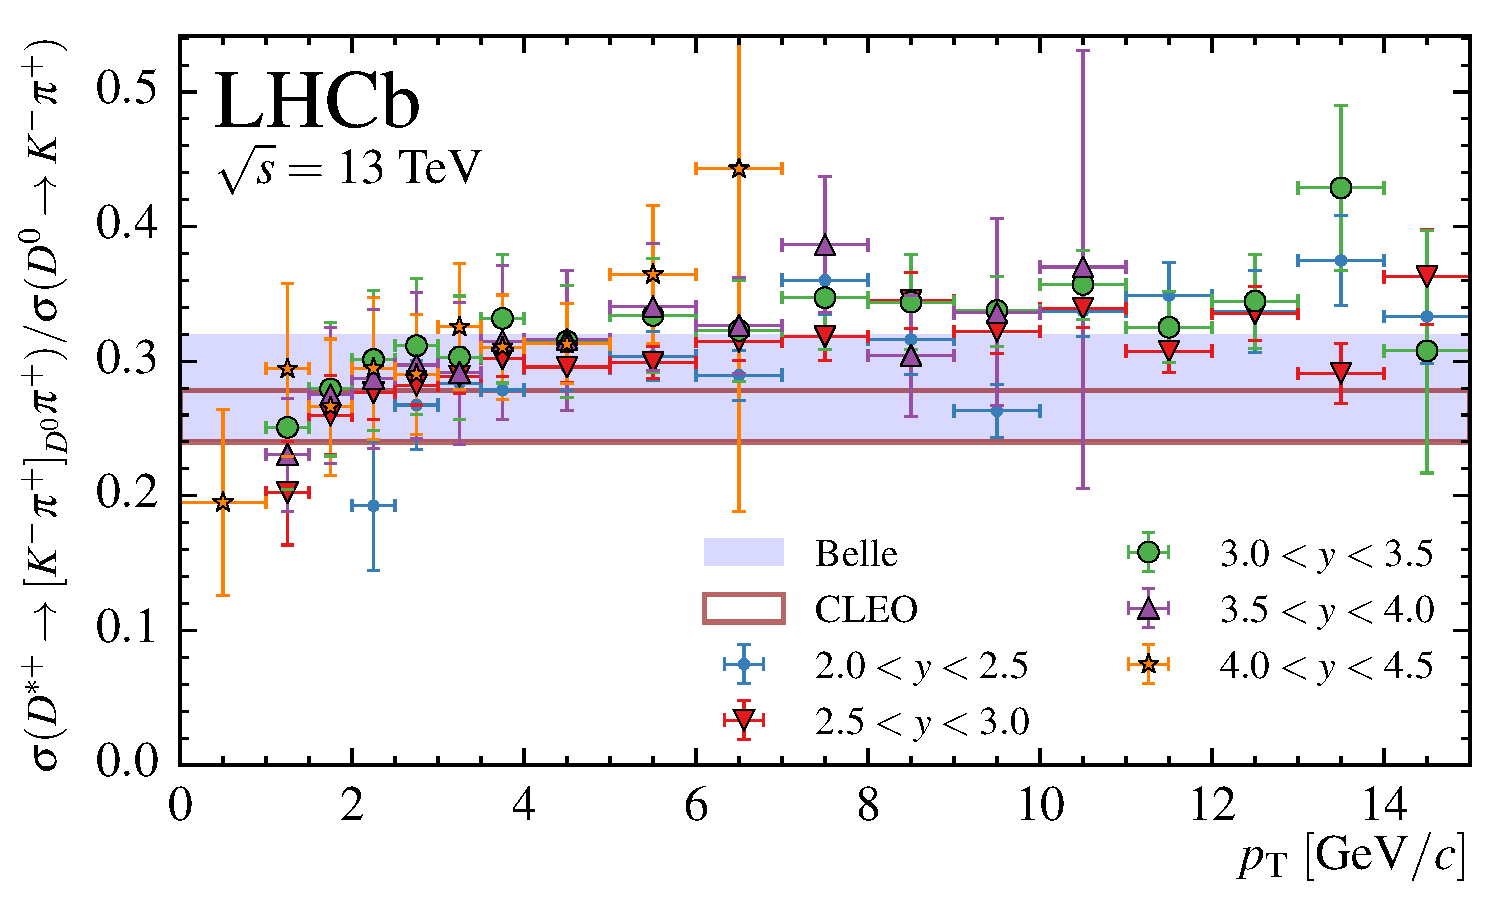
\includegraphics[width=\textwidth]{production/results/Dst_ratio_with_D0}
    \caption{\resultratio{\PDstarp}{\PDzero}}
    \label{fig:prod:results:ratio_mesons:Dst_D0}
  \end{subfigure}
  \caption{%
    Ratios of cross-section times branching fraction measurements of \PDplus
    (\subref*{fig:prod:results:ratio_mesons:Dp_D0}), \PDsplus
    (\subref*{fig:prod:results:ratio_mesons:Ds_D0}), and \PDstarp\
    (\subref*{fig:prod:results:ratio_mesons:Dst_D0}) mesons with respect to the
    \PDzero measurements.
    The bands indicate the corresponding ratios computed using measurements
    from \epem\ collider
    experiments~\cite{Artuso:2004pj,Seuster:2005tr,Aubert:2002ue}.
    The ratios are given as a function of \pT\ and different symbols indicate
    different ranges in \rapidity.
    The notation $\xsec(\HcTof)$ on each $y$-axis is shorthand for
    \xsectimesbfrac.
  }
  \label{fig:prod:results:ratio_mesons_a}
\end{figure}

\begin{figure}
  \begin{subfigure}[b]{0.5\textwidth}
    \centering
    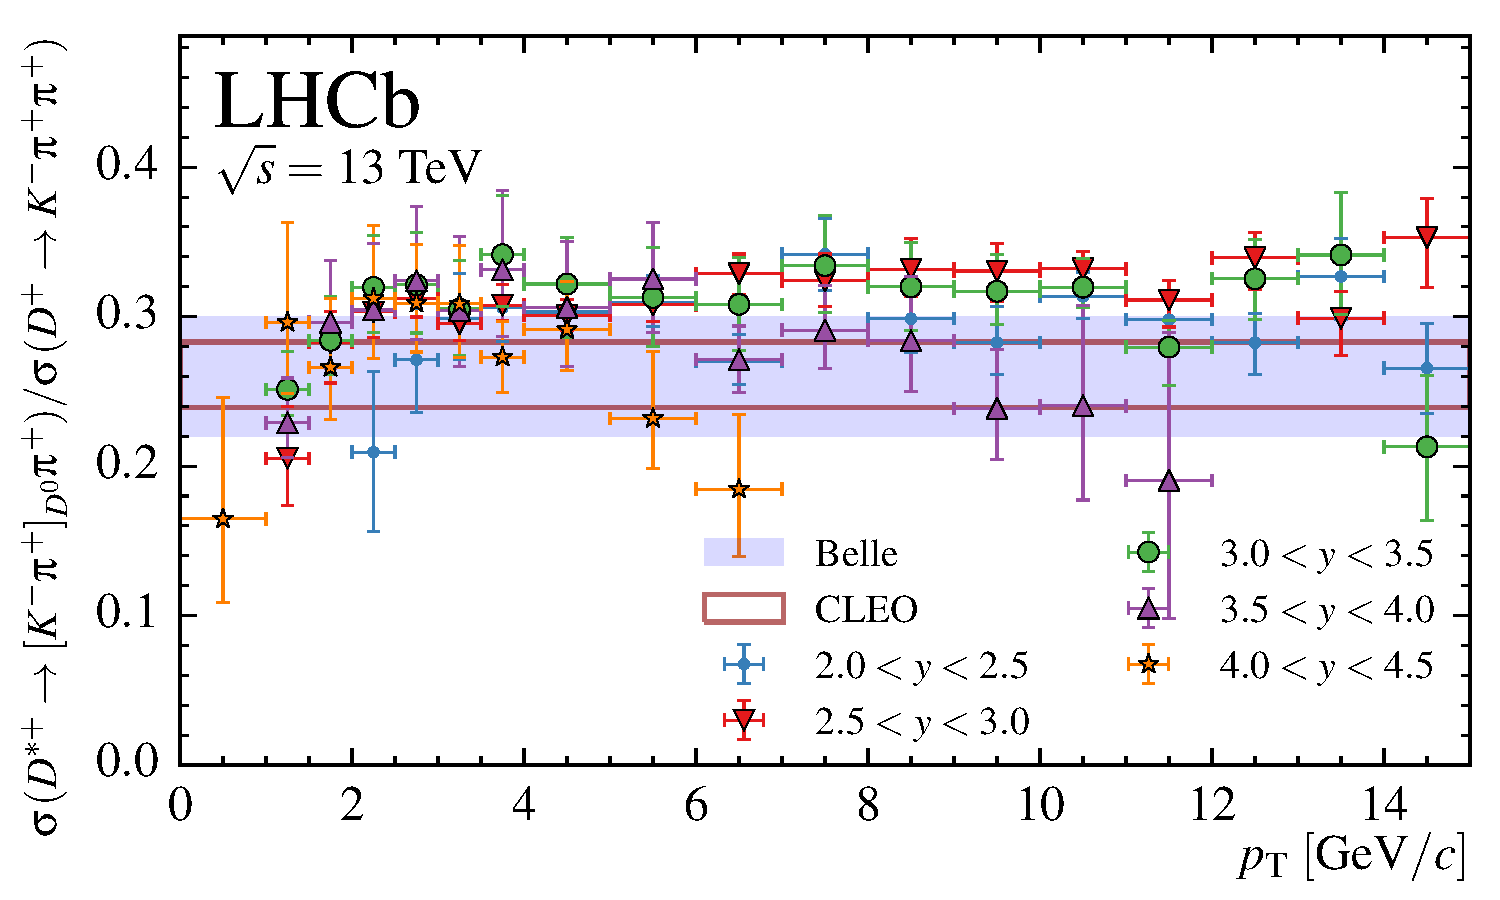
\includegraphics[width=\textwidth]{production/results/Dst_ratio_with_Dp}
    \caption{\resultratio{\PDstarp}{\PDplus}}
    \label{fig:prod:results:ratio_mesons:Dst_Dp}
  \end{subfigure}
  \begin{subfigure}[b]{0.5\textwidth}
    \centering
    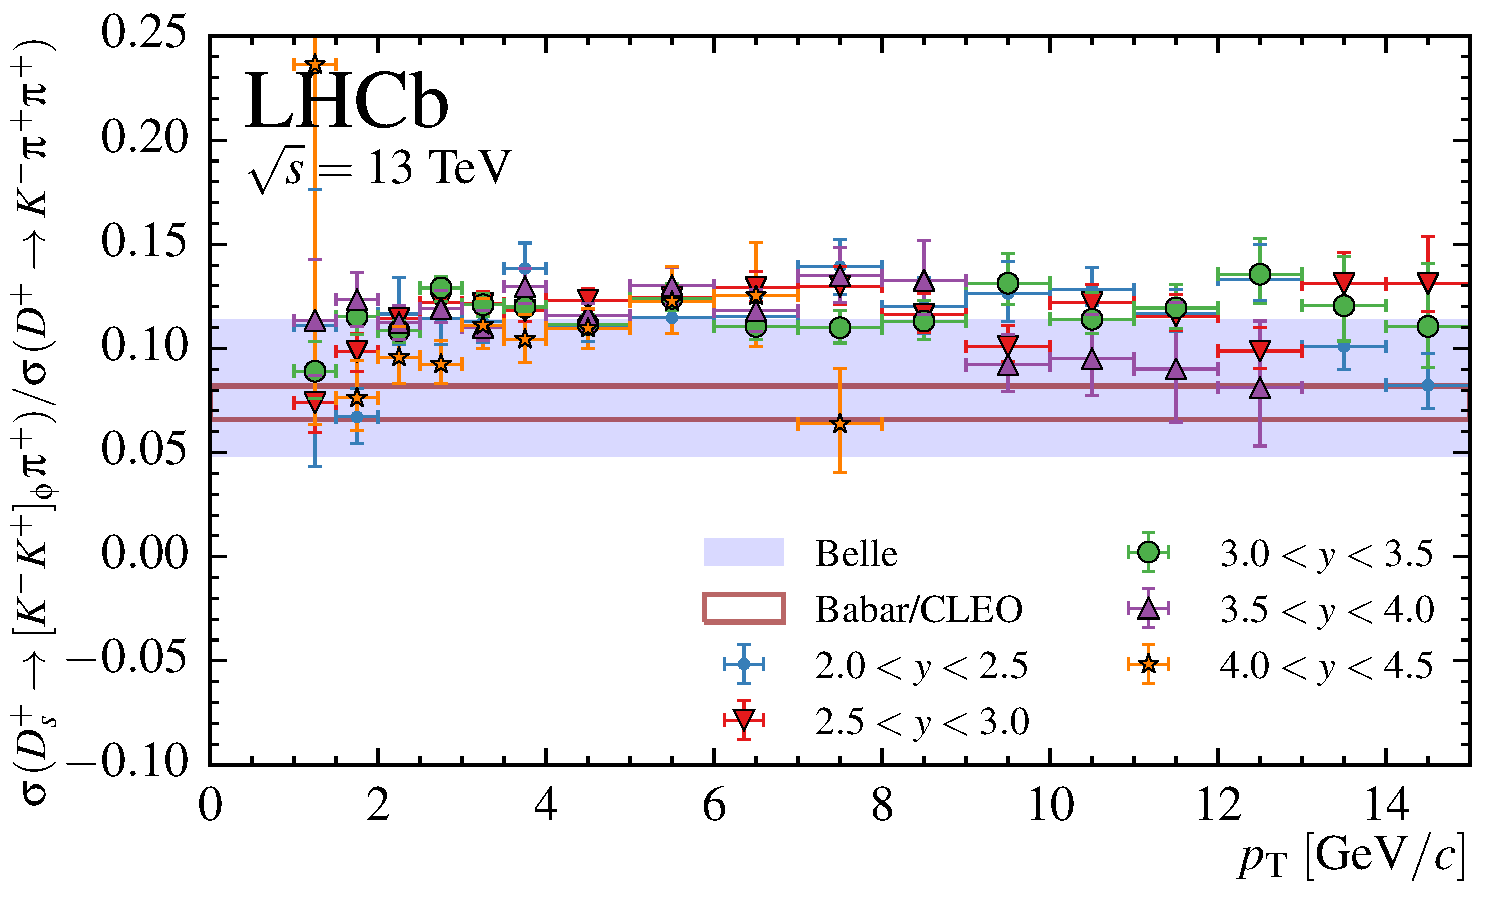
\includegraphics[width=\textwidth]{production/results/Ds_ratio_with_Dp}
    \caption{\resultratio{\PDsplus}{\PDplus}}
    \label{fig:prod:results:ratio_mesons:Ds_Dp}
  \end{subfigure}
  \begin{subfigure}[b]{0.5\textwidth}
    \centering
    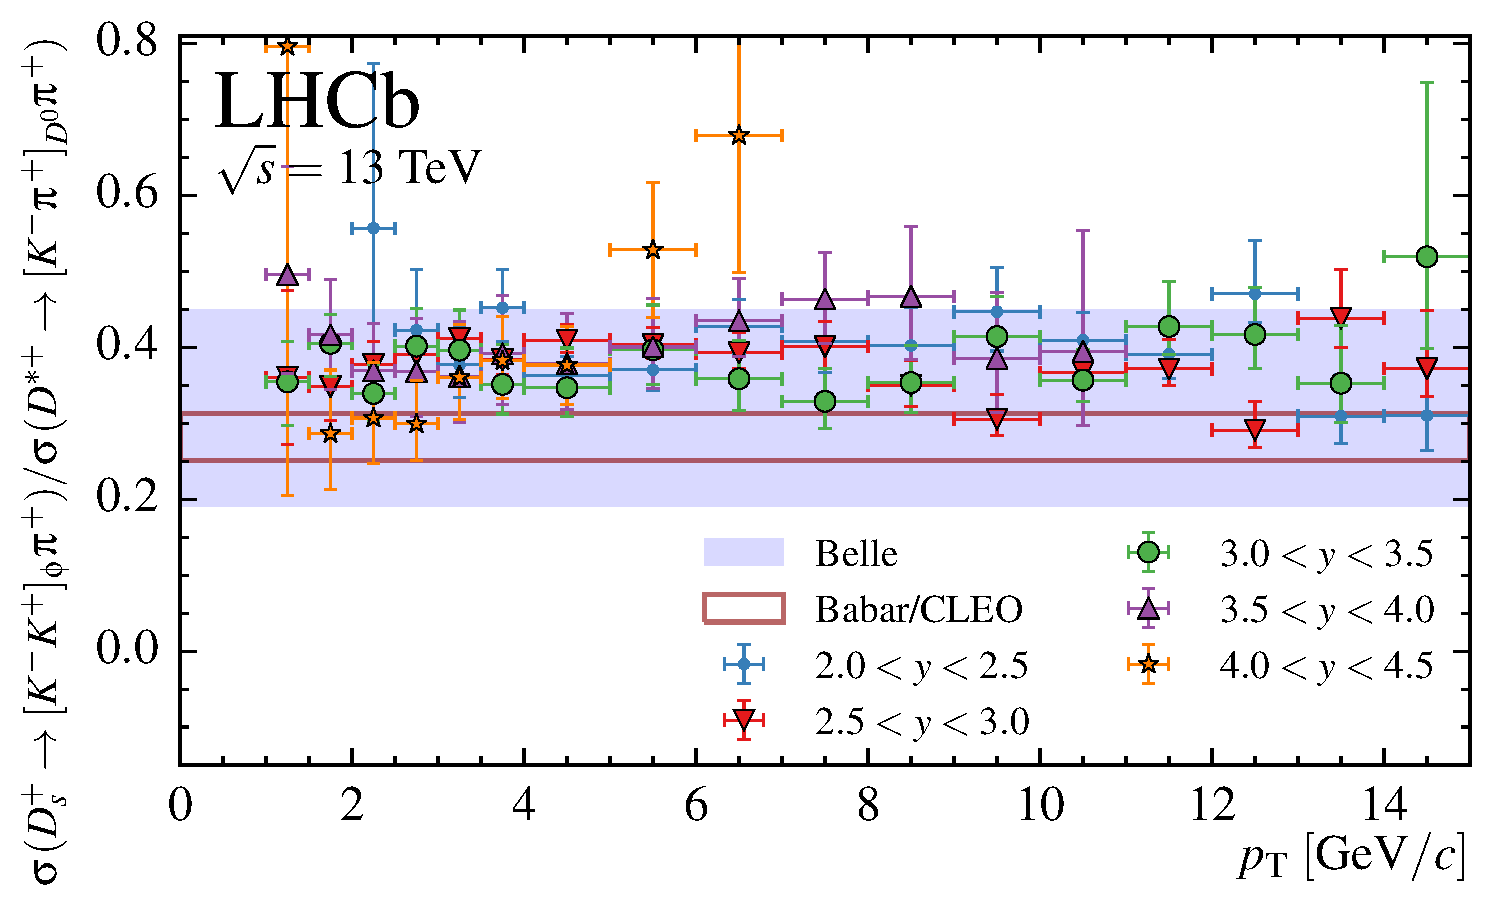
\includegraphics[width=\textwidth]{production/results/Ds_ratio_with_Dst}
    \caption{\resultratio{\PDstarp}{\PDsplus}}
    \label{fig:prod:results:ratio_mesons:Ds_Dst}
  \end{subfigure}
  \caption{%
    Ratios of cross-section times branching fraction measurements for
    $\PDstarp/\PDplus$ (\subref*{fig:prod:results:ratio_mesons:Dst_Dp}),
    $\PDsplus/\PDplus$ (\subref*{fig:prod:results:ratio_mesons:Ds_Dp}), and
    $\PDstarp\PDsplus$ (\subref*{fig:prod:results:ratio_mesons:Ds_Dst}).
    The bands indicate the corresponding ratios computed using measurements
    from \epem\ collider
    experiments~\cite{Artuso:2004pj,Seuster:2005tr,Aubert:2002ue}.
    The ratios are given as a function of \pT\ and different symbols indicate
    different ranges in \rapidity.
    The notation $\xsec(\HcTof)$ on each $y$-axis is shorthand for
    \xsectimesbfrac.
  }
  \label{fig:prod:results:ratio_mesons_b}
\end{figure}

\begin{figure}
  \begin{subfigure}[b]{0.5\textwidth}
    \centering
    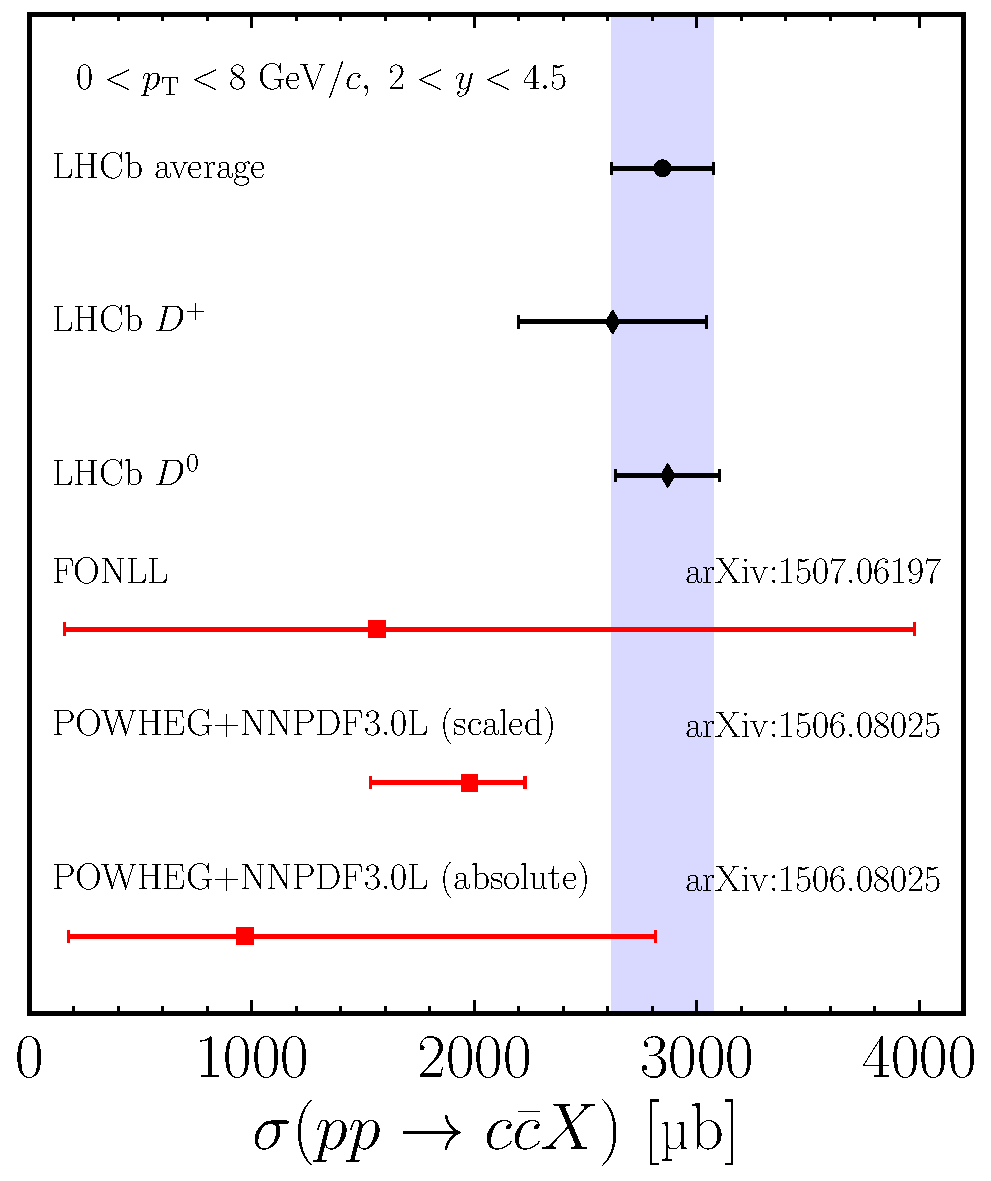
\includegraphics[width=\textwidth]{production/results/integrated_double_differential_0_8}
    \caption{\pTrange{0}{8}}
    \label{fig:prod:results:integrated_double_differential:0_8}
  \end{subfigure}
  \begin{subfigure}[b]{0.5\textwidth}
    \centering
    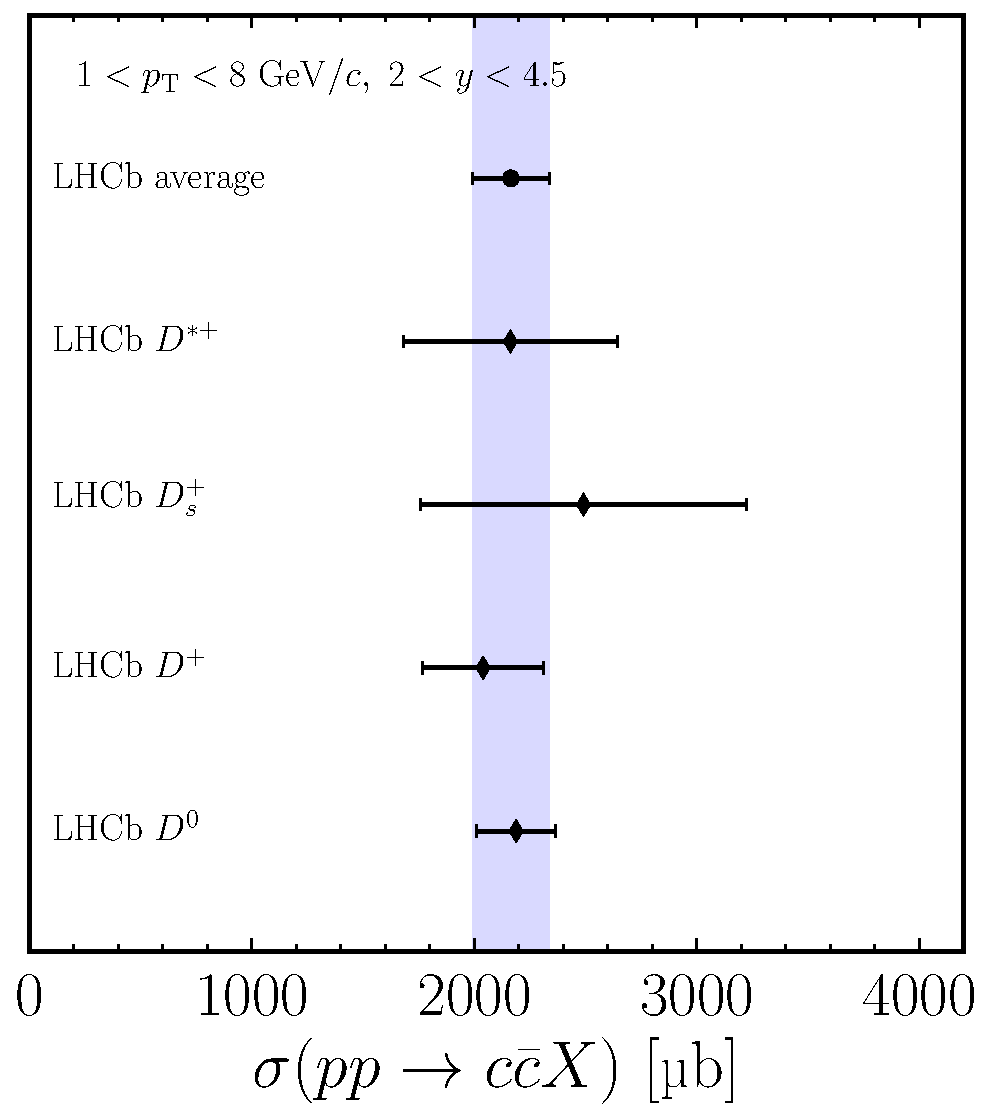
\includegraphics[width=\textwidth]{production/results/integrated_double_differential_1_8}
    \caption{\pTrange{1}{8}}
    \label{fig:prod:results:integrated_double_differential:1_8}
  \end{subfigure}
  \caption{%
    Integrated cross-sections (black diamonds), their average (black circle and
    blue band) and theory predictions (red
    squares)~\cite{Gauld:2015yia,Cacciari:2015fta} are shown based on the
    \PDzero and \PDplus for \pTrange{0}{8}
    (\subref*{fig:prod:results:integrated_double_differential:0_8}) and for
    measurements based on all four mesons for \pTrange{1}{8}
    (\subref*{fig:prod:results:integrated_double_differential:1_8}).
    The ``absolute'' predictions are based on calculations of the \SI{13}{\TeV}
    cross-section, while the ``scaled'' predictions are based on calculations
    of the $13$ to \SI{7}{\TeV} ratio multiplied with the \lhcb\ measurement at
    \SI{7}{\TeV}~\cite{LHCb-PAPER-2012-041}.
  }
  \label{fig:prod:results:integrated_double_differential}
\end{figure}

\begin{table}
  \caption{%
    Prompt charm production cross-sections integrated over \yrange{2}{4.5} and
    the \pT\ ranges given.
    The computation of the extrapolation factors is described in the text.
    The first uncertainty on the cross-section is statistical, and the second
    is systematic and includes the contribution from the extrapolation factor.
    No extrapolation factor is given for $\PD^{+}_{(\Pstrange)}$ as a
    measurement is available in every bin of the integrated phase space.
  }
  \label{tab:prod:results:integrated_double_differential}
  \centering
  \begin{tabular}{ccccr}
  \toprule
           &                  & Extrapolation factor & Cross-section~(\si{\micro\barn}) \\
  \midrule
  \PDzero  & $\pTrange{0}{8}$ & $1.0004 \pm 0.0009$  & $3240 \pm \phantom{1}4 \pm 190$  \\
  \PDplus  & $\pTrange{0}{8}$ & -                    & $1290 \pm \phantom{1}8 \pm 190$  \\
  \midrule
  \PDzero  & $\pTrange{1}{8}$ & $1.0005 \pm 0.0009$  & $2470 \pm \phantom{1}3 \pm 130$  \\
  \PDplus  & $\pTrange{1}{8}$ & -                    & $1000 \pm \phantom{1}3 \pm 110$  \\
  \PDsplus & $\pTrange{1}{8}$ & -                    & $460 \pm 13 \pm 100$             \\
  \PDstarp & $\pTrange{1}{8}$ & $1.0004 \pm 0.0023$  & $880 \pm \phantom{1}5 \pm 140$   \\
  \bottomrule
\end{tabular}

\end{table}

\begin{table}
  \caption{%
    Ratios of integrated cross-section times branching fraction measurements in
    the kinematic range \pTrange{1}{8} and \yrange{2}{4.5}.
    The first uncertainty on the ratio is statistical and the second is
    systematic. The notation $\xsec(\HcTof)$ is shorthand for \xsectimesbfrac.
  }
  \label{tab:prod:results:integrated_meson_ratios}
  \centering
  \renewcommand{\arraystretch}{1.3}
\begin{tabular}{lc}
  \toprule
  Quantity                               & Measurement                                    \\
  \midrule
  $\xsec(\DpToKpipi)/\xsec(\DzToKpi)$    & $0.953 ^{+0.003}_{-0.003}$$^{+0.060}_{-0.054}$ \\
  $\xsec(\DspTophipi)/\xsec(\DzToKpi)$   & $0.106 ^{+0.003}_{-0.003}$$^{+0.009}_{-0.010}$ \\
  $\xsec(\DstToDzpi)/\xsec(\DzToKpi)$    & $0.242 ^{+0.001}_{-0.001}$$^{+0.027}_{-0.026}$ \\
  \midrule
  $\xsec(\DspTophipi)/\xsec(\DpToKpipi)$ & $0.112^{+0.004}_{-0.004}$$^{+0.006}_{-0.009}$  \\
  $\xsec(\DstToDzpi)/\xsec(\DpToKpipi)$  & $0.254^{+0.001}_{-0.001}$$^{+0.016}_{-0.017}$  \\
  \midrule
  $\xsec(\DspTophipi)/\xsec(\DstToDzpi)$ & $0.444^{+0.013}_{-0.013}$$^{+0.042}_{-0.052}$  \\
  \bottomrule
\end{tabular}

\end{table}

% TODO these are in a different style to the rest of the plots
\begin{figure}
  \begin{subfigure}[b]{0.5\textwidth}
    \centering
    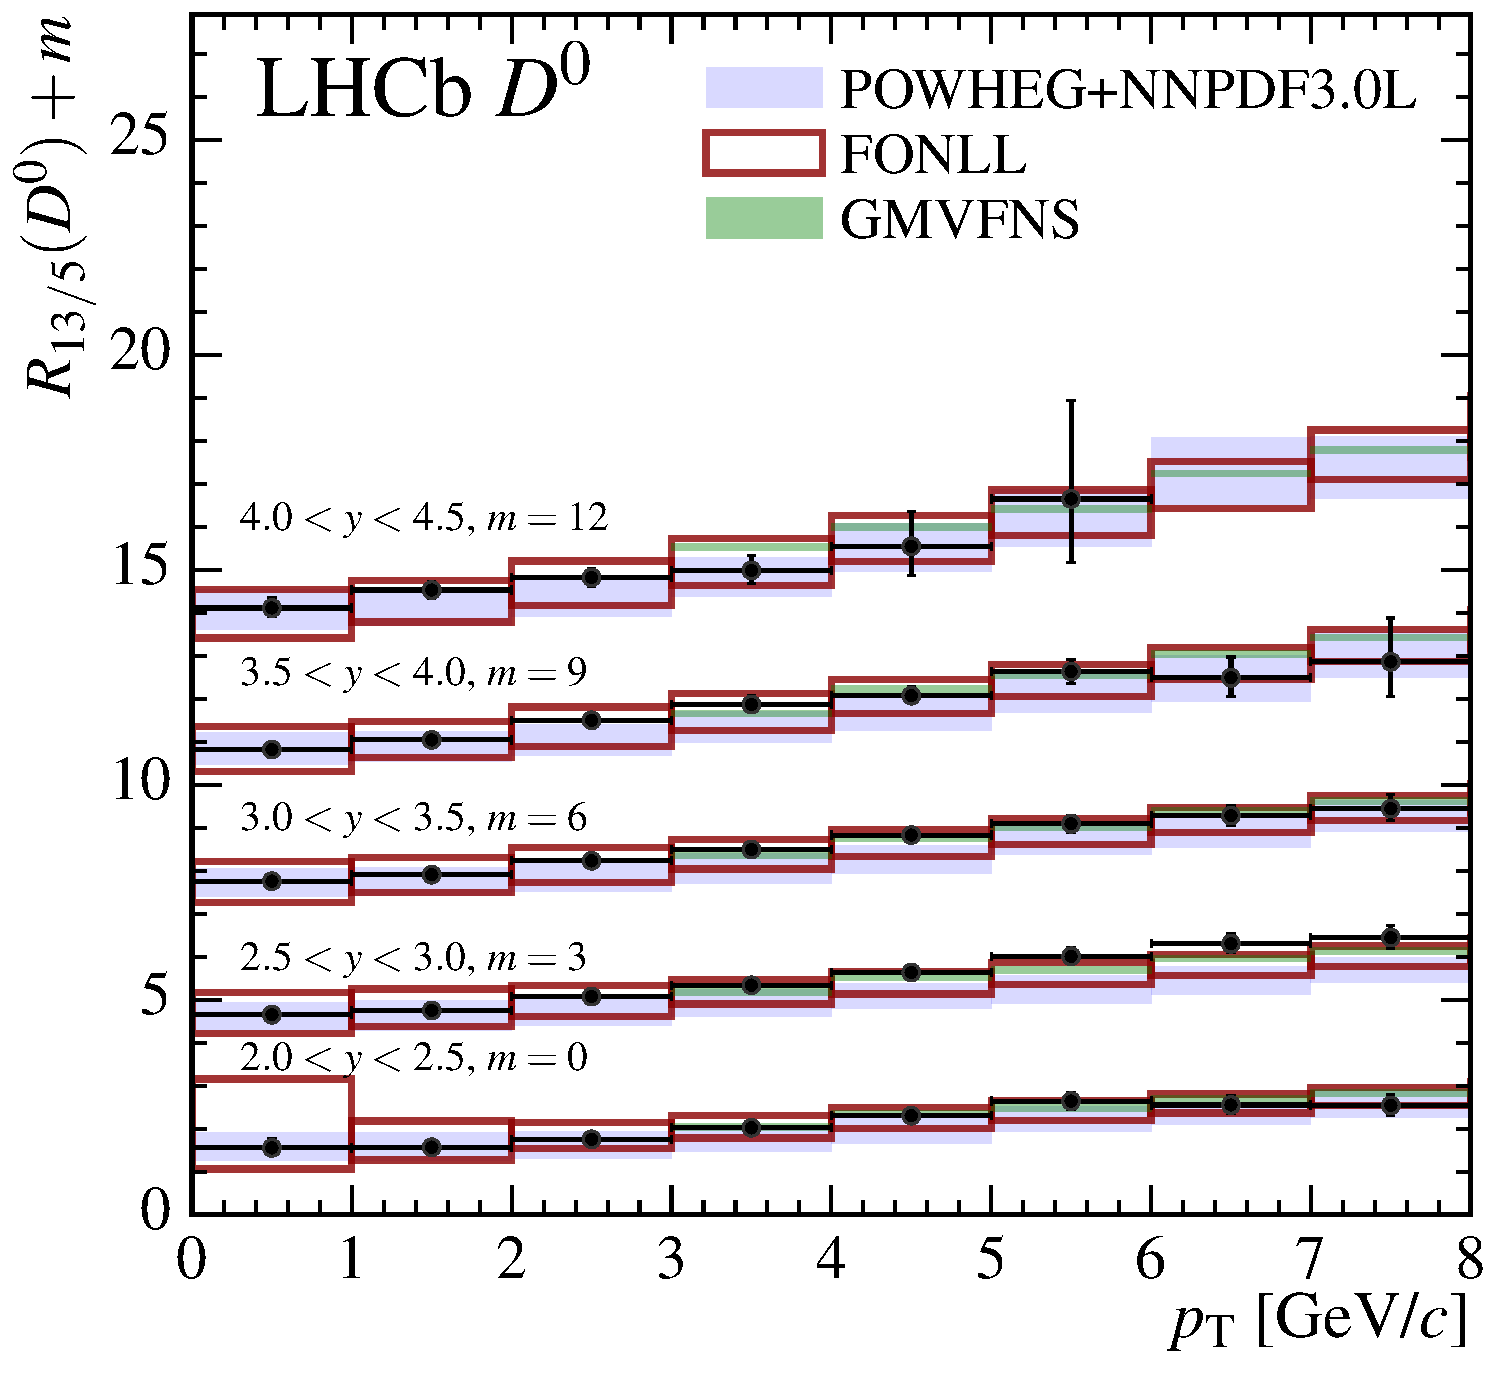
\includegraphics[width=\textwidth]{production/results/D0_ratio_with_2016}
    \caption{\PDzero}
    \label{fig:prod:results:ratio_5tev:D0}
  \end{subfigure}
  \begin{subfigure}[b]{0.5\textwidth}
    \centering
    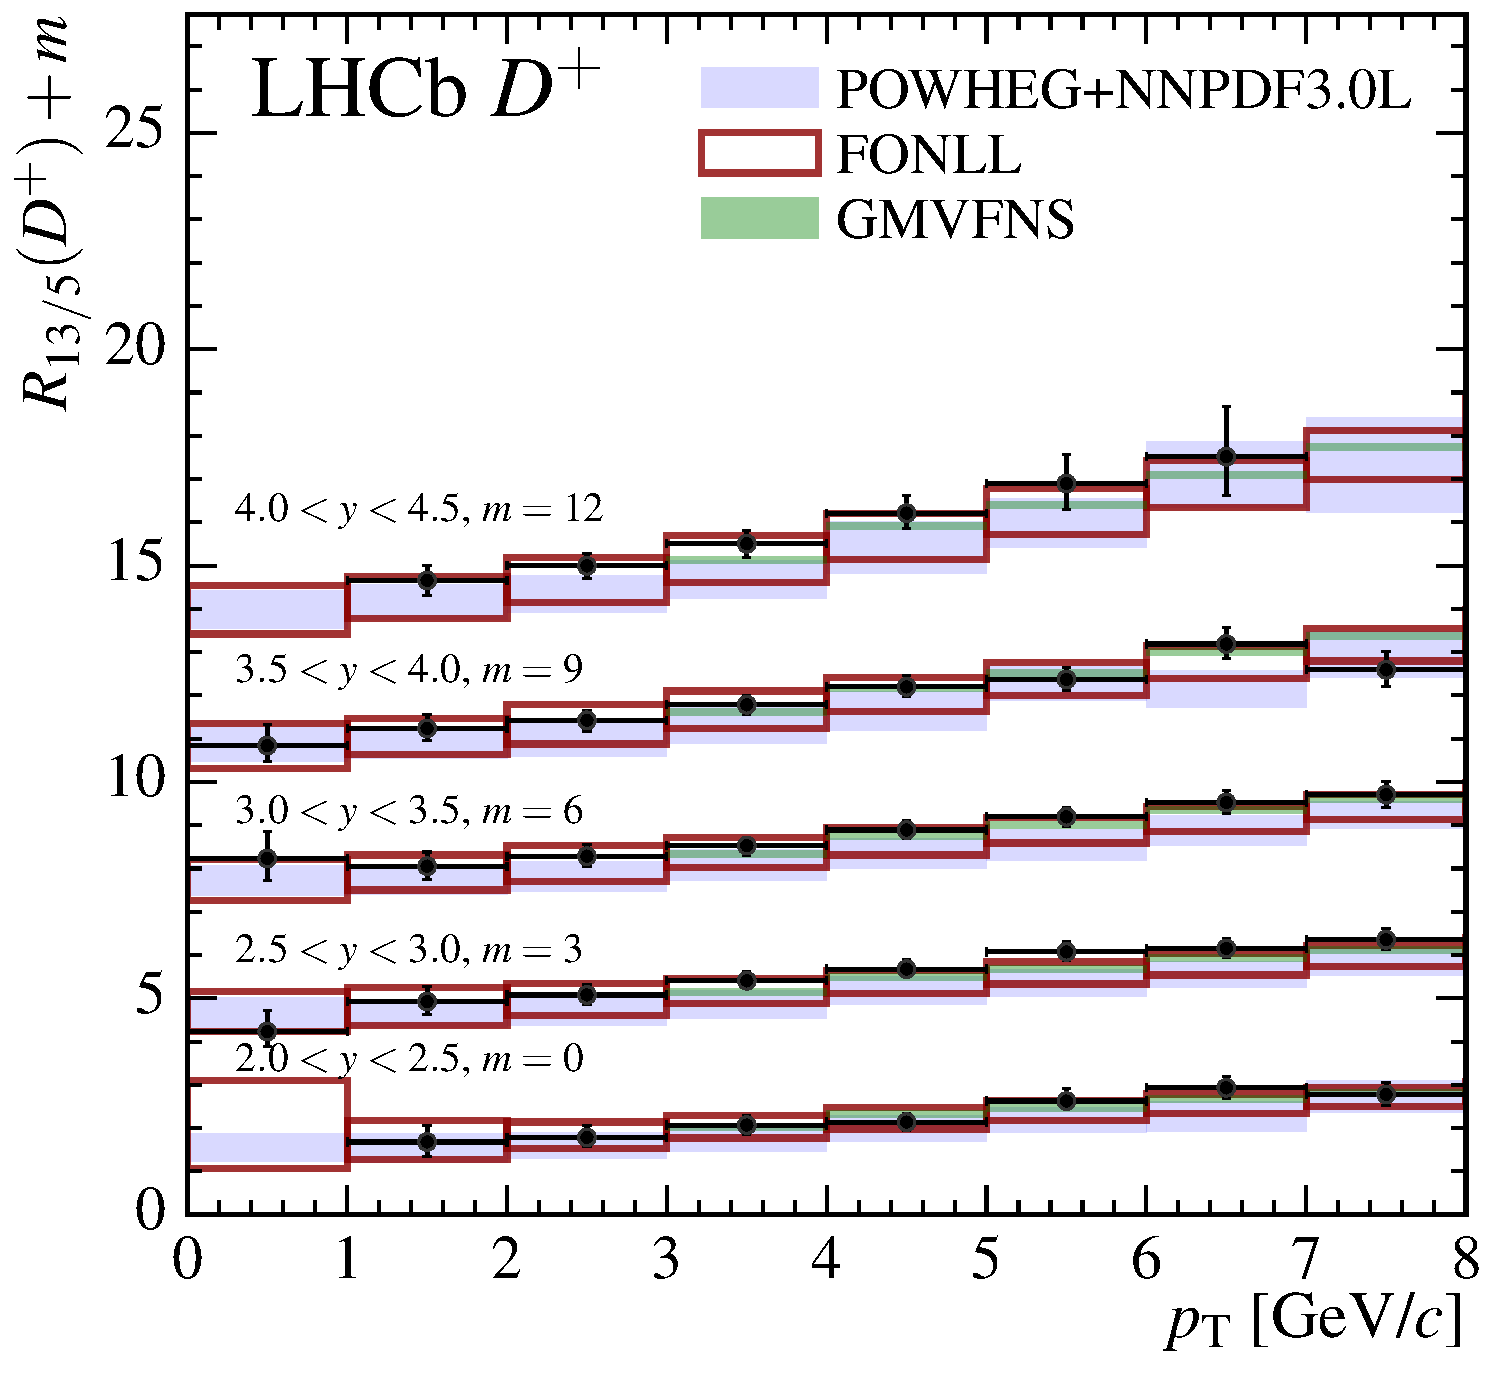
\includegraphics[width=\textwidth]{production/results/Dp_ratio_with_2016}
    \caption{\PDplus}
    \label{fig:prod:results:ratio_5tev:Dp}
  \end{subfigure}
  \begin{subfigure}[b]{0.5\textwidth}
    \centering
    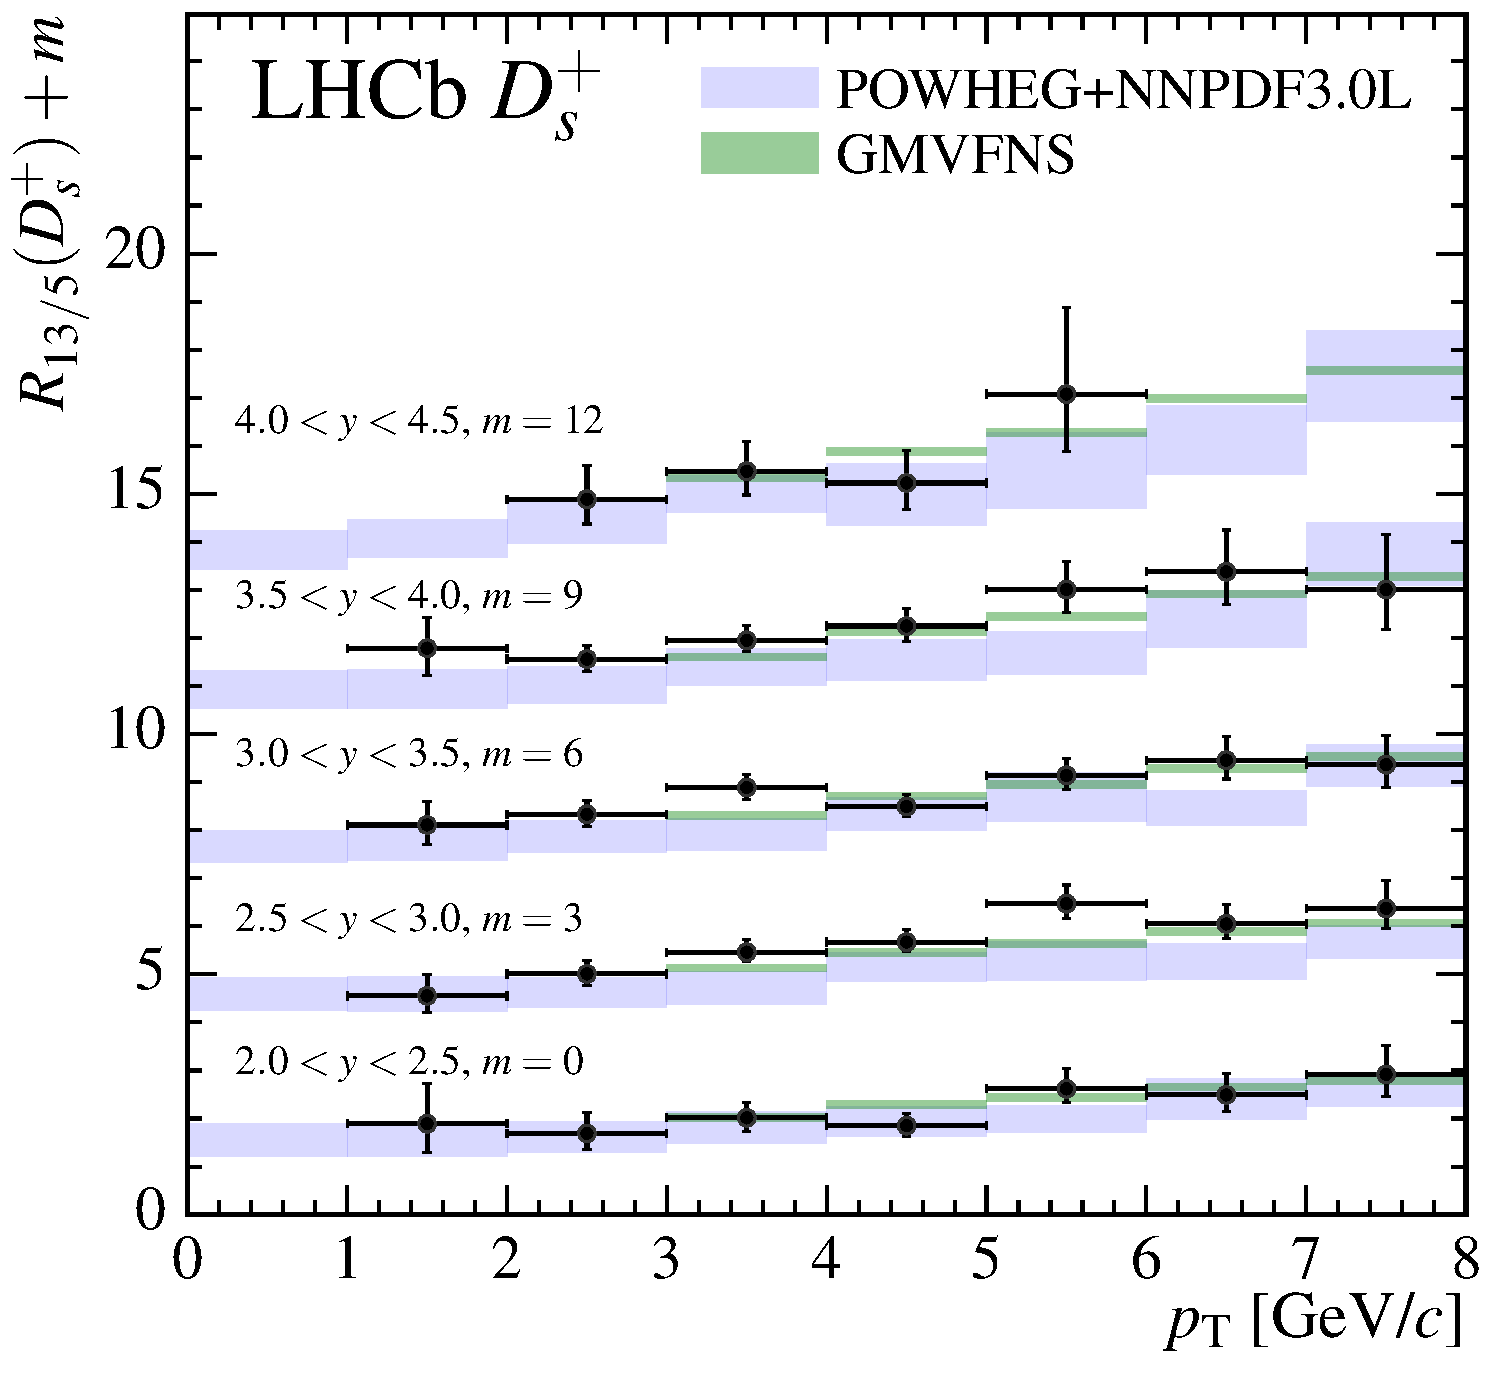
\includegraphics[width=\textwidth]{production/results/Ds_ratio_with_2016}
    \caption{\PDsplus}
    \label{fig:prod:results:ratio_5tev:Ds}
  \end{subfigure}
  \begin{subfigure}[b]{0.5\textwidth}
    \centering
    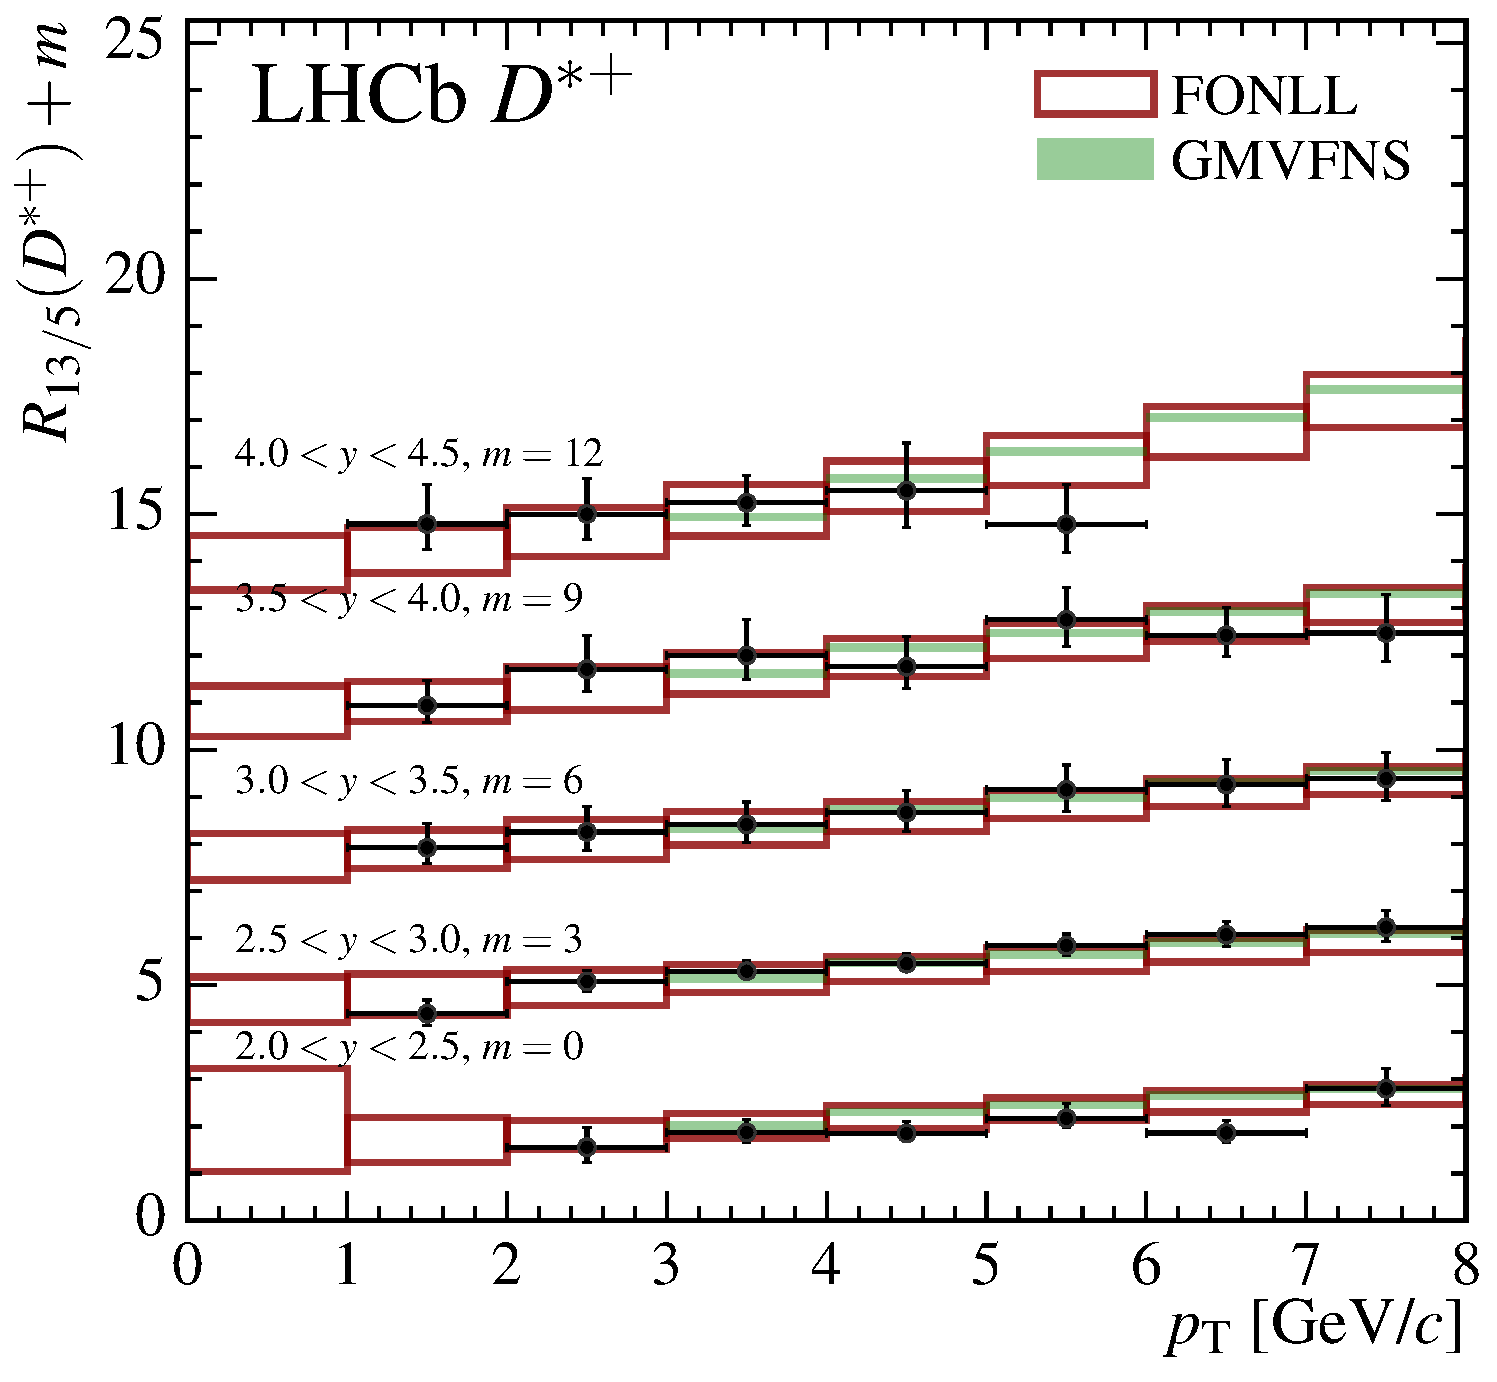
\includegraphics[width=\textwidth]{production/results/Dst_ratio_with_2016}
    \caption{\PDstarp}
    \label{fig:prod:results:ratio_5tev:Dst}
  \end{subfigure}
  \caption{%
    Measurements and predictions of the prompt \PDzero
    (\subref*{fig:prod:results:ratio_5tev:D0}), \PDplus
    (\subref*{fig:prod:results:ratio_5tev:Dp}), \PDsplus
    (\subref*{fig:prod:results:ratio_5tev:Ds}), and \PDstarp
    (\subref*{fig:prod:results:ratio_5tev:Dst}) cross-section ratios
    \resultratio{13}{5}.
    Each set of measurements and predictions in a given rapidity bin is offset
    by an additive factor $m$ shown on the plots.
    The dash-dotted lines indicate the unit ratio for each of the rapidity
    intervals and the dashed lines indicate a ratio of two.
  }
  \label{fig:prod:results:ratio_5tev}
\end{figure}
